\documentclass[xcolor=svgnames, english, smaller]{beamer}
\usetheme{Boadilla}
%\usecolortheme[named=Navy]{structure} 

% input
\usepackage[T1]{fontenc}
\usepackage[latin9]{inputenc}

% math
\usepackage{amsmath, amsthm}

% graphics and figures
\usepackage{graphicx}
\usepackage{subfig}
\usepackage{tikz}
\usetikzlibrary{calc}

\usepackage{algorithm}
\usepackage{algpseudocode}
\usepackage{setspace}

%\setcounter{secnumdepth}{3}
%\setcounter{tocdepth}{3}%\usepackage{xargs}[2008/03/08]
%\usepackage{babel}

%============================================================================================
\theoremstyle{plain}
\newtheorem{thm}{\protect\theoremname}
\theoremstyle{definition}
\newtheorem{defn}[thm]{\protect\definitionname}
\theoremstyle{plain}
\newtheorem{lem}[thm]{\protect\lemmaname}
\theoremstyle{plain}
\newtheorem{cor}[thm]{\protect\corollaryname}

%============================================================================================
% notation
%indices
\global\long\def\itime{k}
\global\long\def\icell{i}
\global\long\def\iconst{h}

\global\long\def\ntime{T}
\global\long\def\ncell{N}
\global\long\def\nconst{8}

%constants
\global\long\def\deltat{\Delta t}
 \global\long\def\deltax{\Delta x}


\global\long\def\prioritysymbol{P}
 \global\long\def\priority#1{\prioritysymbol_{#1}}


%ramps
\global\long\def\rampcontrolsymbol{u}
 \global\long\def\rampcontrol#1#2{\rampcontrolsymbol_{#1}\left(#2\right)}
 \global\long\def\rampcontrolMax#1{\rampcontrolsymbol_{#1}^{\max}}
 \global\long\def\rampqueuesymbol{l}
 \global\long\def\rampqueue#1#2{\rampqueuesymbol_{#1}\left(#2\right)}
 \global\long\def\rampqueueinit#1{\rampqueuesymbol_{#1}^{0}}
 \global\long\def\rampflowsymbol{r}
 \global\long\def\rampflow#1#2{\rampflowsymbol_{#1}\left(#2\right)}


\global\long\def\offrampratiosymbol{\beta}
 \global\long\def\offrampratio#1#2{\offrampratiosymbol_{#1}\left(#2\right)}


%cells
\global\long\def\flowsymbol{f}
 \global\long\def\flowout#1#2{\flowsymbol_{#1}^{\text{out}}\left(#2\right)}
 \global\long\def\flowin#1#2{\flowsymbol_{#1}^{\text{in}}\left(#2\right)}
 

\global\long\def\densitysymbol{\rho}
 \global\long\def\density#1#2{\densitysymbol_{#1}\left(#2\right)}
 \global\long\def\densityinit#1{\densitysymbol_{#1}^{0}}


%input
\global\long\def\inputfluxsymbol{D}
 \global\long\def\inputflux#1#2{D_{#1}\left(#2\right)}


%supply and demand
\global\long\def\celldemandsymbol{\delta}
 \global\long\def\celldemand#1#2{\celldemandsymbol_{#1}\left(#2\right)}


\global\long\def\cellsupplysymbol{\sigma}
 \global\long\def\cellsupply#1#2{\cellsupplysymbol_{#1}\left(#2\right)}


\global\long\def\rampdemandsymbol{d}
 \global\long\def\rampdemand#1#2{\rampdemandsymbol_{#1}\left(#2\right)}


%parameters
\global\long\def\ffspeedsymbol{v}
 \global\long\def\ffspeed#1{\ffspeedsymbol_{#1}}


\global\long\def\congspeedsymbol{w}
 \global\long\def\congspeed#1{\congspeedsymbol_{#1}}


\global\long\def\fmaxsymbol{F}
 \global\long\def\fmax#1{\fmaxsymbol_{#1}}


\global\long\def\jamdensitysymbol{\densitysymbol^{\text{jam}}}
 \global\long\def\jamdensity#1{\jamdensitysymbol_{#1}}


%adjoint
\global\long\def\state#1#2{x_{#1}\left( #2 \right)}
\global\long\def\ind#1{1_{\left\{#1\right\}}}

\global\long\def\stdidx#1{#1{\itime}{\icell}}
\global\long\def\sstdidx#1{\stdidx{#1{\iconst}}}

\global\long\def\H#1#2#3{H^{#1}_{#2, #3}}
\global\long\def\stdH#1{\stdidx{\H{#1}}}
\global\long\def\sstdH{\sstdidx{\H}}

\global\long\def\G#1#2#3{G^{#1}_{#2, #3}}
\global\long\def\stdG#1{\stdidx{\G{#1}}}
\global\long\def\sstdG{\sstdidx{\G}}

\global\long\def\Lambd#1#2#3{\lambda^{#1}_{#2, #3}}
\global\long\def\stdLambd#1{\stdidx{\Lambd{#1}}}
\global\long\def\sstdLambd{\sstdidx{\Lambd}}

\global\long\def\R#1#2#3{R{#1}_{#2, #3}}

% Riemann problem
\global\long\def\rs{\mathcal{RS}}
\global\long\def\js{\mathcal{JS}}


% math commands
\newcommand \eqv{\Leftrightarrow}
\newcommand \Rbb{\mathbb{R}}
\newcommand \Ucal{\mathcal{U}}
\newcommand \Xcal{\mathcal{X}}
\newcommand \Fontvi{\fontsize{8}{8}\selectfont}
\newcommand \FontSmall{\fontsize{6}{6}\selectfont}
\newcommand \FontSmaller{\fontsize{5}{6}\selectfont}
\newcommand \systemDiagOffset{-1.8in}
\newcommand \systemDiagResizeMult{1.3}

% operators


%============================================================================================
\begin{document}

\title{Adjoint-based Control of Traffic Systems\\
Application to Ramp Metering }
\author{Samitha Samaranayake \and Walid Krichene \\ Jack Reilly \and Maria-Laura Delle Monache}
\institute{}
\date{November 21, 2012}

%-----------------------------------------------------------------------------------------------------------------------------------------------------------------

\begin{frame}
\titlepage
\end{frame}

%-----------------------------------------------------------------------------------------------------------------------------------------------------------------
\begin{frame}{Outline}
\tableofcontents
\end{frame}

\AtBeginSubsection[]{
\begin{frame}<beamer>\frametitle{Outline}
\tableofcontents[currentsubsection] 
\end{frame}
}

%============================================================================================
\section{Introduction to the adjoint method}
\subsection{Optimization of a PDE-constrained system}
%-----------------------------------------------------------------------------------------------------------------------------------------------------------------


\begin{frame}{Optimization of a PDE-constrained system}

\begin{block}{Optimization problem}
\[
\begin{aligned}
&\text{minimize}_{u \in \Ucal} && J(x,u) \\
&\text{subject to} &&H(x,u) = 0
\end{aligned}
\]
\end{block}

\begin{itemize}
\item $x \in \Xcal \subseteq \Rbb^n$: state variables
\item $u \in \Ucal  \subseteq \Rbb^m$: control variables
\end{itemize}


\[
\begin{aligned}
J: \Xcal \times \Ucal & \rightarrow \mathbb{R}\\
(x,u) & \mapsto J(x,u)
\end{aligned}
\]

\[
\begin{aligned}
H: \Xcal \times \Ucal & \rightarrow \mathbb{R}^{n_H}\\
(x,u) & \mapsto H(x,u)
\end{aligned}
\]

Want to do gradient descent. How to compute the gradient?
\end{frame}


%-----------------------------------------------------------------------------------------------------------------------------------------------------------------
\subsection{Example: linear system}

\begin{frame}{Example: linear system}
\begin{block}{Discrete linear dynamics}
\[
x_{t+1} = A x_t + B u_t, \ t \in \{0, \dots, T-1 \}
\]
with initial condition $x_0$.
\end{block}

Let
\begin{align*}
& x = \left[ \begin{array}{c} x_1 \\ \vdots \\ x_T \end{array}\right] && u = \left[ \begin{array}{c} u_0 \\ \vdots \\ u_{T-1} \end{array}\right]
\end{align*}
%

\end{frame}



%-----------------------------------------------------------------------------------------------------------------------------------------------------------------
\begin{frame}{Example: linear system}

\begin{align*}
x &= 
\left[
\begin{array}{c}
A x_0 + B u_0 \\
A x_1 + B u_1 \\
\vdots \\
A x_{T-1} + B u_{T-1}
\end{array}
\right] \\
& =
\left[
\begin{array}{cccc} 
0 &             &            & \\
A & \ddots &           & \\
   & \ddots & \ddots& \\
   &            & A         & 0 
\end{array}
\right]
x + 
\left[\begin{array}{cccc}
B &             &            & \\
   & \ddots &             & \\
   &             & \ddots & \\
   &             &              &B
\end{array} \right]
u + 
\left[\begin{array}{c}
A x_0 \\
0 \\
\vdots \\
0
\end{array}\right]
\end{align*}

Can be written as 
\[
(\tilde{A} - I)x + \tilde{B} u + c = 0
\]

Note: $(\tilde{A} - I)$ is invertible (lower triangular, with $-1$ on diagonal). Good: system is deterministic!

\end{frame}



%-----------------------------------------------------------------------------------------------------------------------------------------------------------------

\newcommand \xuVector{\left[\begin{array}{c} x \\ u \end{array} \right]}
\begin{frame}{Example: linear system}

\begin{block}{Linear system}
\[
H_x x + H_u u + c = 0
\]
\end{block}

\begin{itemize}
\item $x \in \Rbb^{n}$ state
\item $u \in \Rbb^{m}$ control, with $m \leq n$
\item $H_x \in \Rbb^{n \times n}$, assume invertible
\item $H_u \in \Rbb^{n \times m}$
\item $c \in \Rbb^n$
\end{itemize}

want to minimize linear cost function
\[
\begin{aligned}
&\text{minimize}_{u \in \Ucal} && J_x x + J_u u \\
&\text{subject to} && H_x x + H_u u + c = 0
\end{aligned}
\]

$J_x \in \Rbb^{1\times n}$ and $J_u \in \Rbb^{1 \times m}$ are given row vectors.

\end{frame}

%-----------------------------------------------------------------------------------------------------------------------------------------------------------------

\begin{frame}{Example: linear system}

\begin{block}{Optimization problem}
\[
\begin{aligned}
&\text{minimize}_{u \in \Ucal} && J_x x + J_u u \\
&\text{subject to} && H_x x + H_u u + c = 0
\end{aligned}
\]
\end{block}
An equivalent problem is
\[
\text{minimize}_{u \in \Ucal} - J_x H_x^{-1}(H_u u + c) + J_u u
\]
and the gradient is
\begin{block}{Gradient}
\[
\nabla_u J = \alert{- J_x H_x^{-1} H_u} + J_u
\]
\end{block}

\end{frame}

%-----------------------------------------------------------------------------------------------------------------------------------------------------------------
\begin{frame}{Example: linear system}
\small
\begin{block}{Gradient}
\[
\nabla_u J = - J_x H_x^{-1} H_u + J_u
\]
\end{block}
Two ways to compute the first term

\begin{minipage}[t]{0.50\textwidth}
\small
\begin{block}{Forward}
\[
\begin{aligned}
& J_x \alert{M} \\
& H_x \alert{M} = - H_u
\end{aligned}
\]
\end{block}
Solve for $\alert{M \in \Rbb^{n \times m}}$: $m$ inversions
\[
H_x \left[\begin{array}{c|c|c} M_1 & \dots & M_m \end{array} \right] = \left[\begin{array}{c|c|c} H_{u_1} & \dots & H_{u_m} \end{array} \right]
\]
Cost $O(mn^2)$.\\
Then product $1\times n$ times $n \times m$: $O(nm)$

\end{minipage}\hfill
%------------------------------------------------------------------------------
\begin{minipage}[t]{0.46\textwidth}
\small
\begin{block}{Adjoint}
\[
\begin{aligned}
& {\color{Green}\lambda^T} H_u \\
& {\color{Green}\lambda^T} H_x = -J_x
\end{aligned}
\]
\end{block}
Solve for $\color{Green} \lambda \in \Rbb^{n} $: $1$ inversion
\[
H_x^T \lambda = J_x^T
\]
Cost $O(n^2)$.\\
Then product $1\times n$ times $n \times m$: $O(nm)$

\end{minipage}

\end{frame}

%-----------------------------------------------------------------------------------------------------------------------------------------------------------------
\subsection{Solving the original problem}



\begin{frame}{Optimization of a PDE-constrained system}
\small
%------------------------------------------------------------------------------
\begin{minipage}[t]{0.44\textwidth}
\begin{block}{General problem}
\[
\begin{aligned}
&\text{minimize}_{u \in \Ucal} && J(x,u) \\
&\text{subject to} &&H(x,u) = 0
\end{aligned}
\]
\end{block}
\vspace{-0.2cm}
\[
\nabla_u J = \frac{\partial J}{\partial x} \alert{\nabla_u x} + \frac{\partial J}{\partial u}
\]
On trajectories, $H(x, u) = 0$ constant, thus $\nabla_u H = 0$
\[
\frac{\partial H}{\partial x} \alert{\nabla_u x} + \frac{\partial H}{\partial u} = 0
\]
\vspace{-0.5cm}
\uncover<3>{
\begin{block}{Adjoint}
\[
\frac{\partial H}{\partial x}^T {\color{Green}\lambda} = \frac{\partial J}{\partial x}
\]
\end{block}
then
\[
\nabla_u J = {\color{Green}\lambda^T} \frac{\partial H}{\partial u} + \frac{\partial J}{\partial u}
\]
}
\end{minipage}\hfill
%------------------------------------------------------------------------------
\begin{minipage}[t]{0.52\textwidth}
\begin{block}{Linear system}
\[
\begin{aligned}
&\text{minimize}_{u \in \Ucal} && J_x x + J_u u \\
&\text{subject to} && H_x x + H_u u + c = 0
\end{aligned}
\]
\end{block}
\vspace{-0.2cm}
\[
\nabla_u J = J_x \alert{M} + J_u
\]
\vspace{0.9cm}
\[
H_x \alert{M} = - H_u
\]
\uncover<2, 3>{
Instead, solve for $\color{Green}\lambda \in \Rbb^{n}$
\begin{block}{Adjoint}
\[
H_x^T {\color{Green}\lambda} = J_x^T
\]
\end{block}
then
\[
\nabla_u J = {\color{Green}\lambda^T} H_u + J_u
\]
}
\end{minipage}



\end{frame}


%-----------------------------------------------------------------------------------------------------------------------------------------------------------------

\begin{frame}{Computing $\nabla_u J(x, u)$}

Want to evaluate
\begin{align*}
&\frac{\partial J}{\partial x} \alert{\nabla_u x} \\
&\text{where } \frac{\partial H}{\partial x} \alert{\nabla_u x} + \frac{\partial H}{\partial u} = 0
\end{align*}

\pause If $\lambda$ is solution to the adjoint equation
\[
\frac{\partial J}{\partial x} + {\color{Green}\lambda^T} \frac{\partial H}{\partial x} = 0
\]
\pause Then
\[
\frac{\partial J}{\partial x} \alert{\nabla_u x} = -{\color{Green}\lambda^T} \frac{\partial H}{\partial x} \alert{\nabla_u x} = {\color{Green}\lambda^T} \frac{\partial H}{\partial u}
\]

\end{frame}

%-----------------------------------------------------------------------------------------------------------------------------------------------------------------
\begin{frame}{Adjoint solution $\lambda$}

\[
\nabla_u J = \lambda^T \frac{\partial H}{\partial u} + \frac{\partial J}{\partial u}
\]

Also useful for sensitivity analysis.

\begin{block}{Sensitivity analysis}
$\lambda_k$ is the price of changing $H_k$
\end{block}


\end{frame}


%============================================================================================
\section{Discretized system dynamics}

%-----------------------------------------------------------------------------------------------------------------------------------------------------------------
\subsection{Forward System}
\begin{frame}{Forward system}

%\begin{figure}[h]
%\centering
%\resizebox{\columnwidth}{!}{

\begin{tikzpicture}[scale=1.4]

\def \linkWidth {1cm}
\def \nodeWidth {0.3cm}

\coordinate (arrow) at (1.8,0);
\coordinate (dots) at (0.5,0);
\coordinate (unit) at (2.5,0);

\node (link0) at (0,0) [rectangle, minimum width=\linkWidth, draw] {$0$};
\node (link1) at ($(link0) + 1*(unit)$) [rectangle, minimum width=\linkWidth, draw] {$1$};
\node (linkI) at ($(link1) + 2*(unit)$) [rectangle, minimum width=\linkWidth, draw] {$\icell$};
\node (nodeI) at ($(linkI) + 1*(unit)$) [circle, minimum width=\nodeWidth, draw] {$\icell$};

\node (onrampI) at ($(linkI)-(0,0.8)$) [rectangle, minimum width=\linkWidth, draw] {on-ramp $\icell$};
\node (offrampI) at ($(linkI) + 1.4*(unit) - (0,0.5)$) {};

\node (linkI1) at ($(nodeI) + 1.45*(unit)$) [rectangle, minimum width=\linkWidth, draw] {$\icell+1$};

\node (linkN) at ($(linkI1)+1.8*(unit)$) [rectangle, minimum width=\linkWidth, draw] {$\ncell$};

% link 0
\draw[->] ($(link0)-(arrow)$) -- (link0) node[above, midway] {$\inputflux{0}{\itime}$};
\draw[->] (link0) -- (link1) node[above, midway] {$\flowout{0}{\itime}$};

% link 1
\draw[->] (link1) -- ($(link1) + (arrow)$) node[above, midway] {$\flowout{1}{\itime}$};

%dots
\draw ($(link1) + (arrow) + (dots)$) node{$\dots$} ;

% link i
\draw[->] ($(linkI) - 1.3*(arrow)$) -- (linkI)node[above, xshift=-1.1cm] {$\flowin{\icell}{\itime}$};
\draw[->] (linkI) -- (nodeI) node[above, midway] {$\flowout{\icell}{\itime}$};
\draw[->] (nodeI) -- (linkI1) node[above, xshift=-1.1cm]{$\flowin{\icell+1}{\itime}$} ;

%node i
\draw[->] (onrampI) [anchor=right]-- (nodeI) node[below, midway]{$\rampflow{\icell}{\itime}$};
\draw[->] ($(onrampI) - (arrow)$) [anchor=right]-- (onrampI) node[above, midway]{$\inputflux{\icell}{\itime}$};
\draw[->] (nodeI) -- (offrampI) node[below, xshift=-0.3cm]{$\offrampratio{\icell}{\itime} \flowout{\icell}{\itime}$};

%link i+1
\draw[->] (linkI1) -- ($(linkI1) + (arrow)$) node[above, midway] {$\flowout{\icell+1}{\itime}$};

%dots
\draw ($(linkI1)+(arrow)+(dots)$) node{$\dots$} ;

% link N
\draw[->] ($(linkN) - (arrow)$) -- (linkN) node[above, midway] {$\flowin{\ncell}{\itime}$};
\draw[->] (linkN)--($(linkN) + (arrow)$) node[above, midway] {$\flowout{\ncell}{\itime}$};

% box
\draw[dashed] ($(linkI) + (-2,1)$) rectangle ($(nodeI) + (1.8,-1.5)$) node[below]{block $\icell$};

\end{tikzpicture}
}
%\caption{Discrete system}
%\label{fig:system}
%\end{figure}

\begin{figure}[t]
\hspace{\systemDiagOffset}
\resizebox{\systemDiagResizeMult\columnwidth}{!}{%indices
\global\long\def\itime{k}
\global\long\def\icell{i}
\global\long\def\iconst{h}

\global\long\def\ntime{T}
\global\long\def\ncell{N}
\global\long\def\nconst{8}

%constants
\global\long\def\deltat{\triangle t}
\global\long\def\deltax{\triangle x}


\global\long\def\prioritysymbol{P}
 \global\long\def\priority#1{\prioritysymbol_{#1}}


%ramps
\global\long\def\rampcontrolsymbol{u}
 \global\long\def\rampcontrol#1#2{\rampcontrolsymbol_{#1}\left(#2\right)}
 \global\long\def\rampcontrolMax#1{\rampcontrolsymbol_{#1}^{\max}}
 \global\long\def\rampqueuesymbol{l}
 \global\long\def\rampqueue#1#2{\rampqueuesymbol_{#1}\left(#2\right)}
 \global\long\def\rampqueueinit#1{\rampqueuesymbol_{#1}^{0}}
 \global\long\def\rampflowsymbol{r}
 \global\long\def\rampflow#1#2{\rampflowsymbol_{#1}\left(#2\right)}


\global\long\def\offrampratiosymbol{\beta}
 \global\long\def\offrampratio#1#2{\offrampratiosymbol_{#1}\left(#2\right)}


%cells
\global\long\def\flowsymbol{f}
 \global\long\def\flowout#1#2{\flowsymbol_{#1}^{\text{out}}\left(#2\right)}
 \global\long\def\flowin#1#2{\flowsymbol_{#1}^{\text{in}}\left(#2\right)}
 

\global\long\def\densitysymbol{\rho}
 \global\long\def\density#1#2{\densitysymbol_{#1}\left(#2\right)}
 \global\long\def\densityinit#1{\densitysymbol_{#1}^{0}}


%input
\global\long\def\inputfluxsymbol{D}
 \global\long\def\inputflux#1#2{D_{#1}\left(#2\right)}


%supply and demand
\global\long\def\celldemandsymbol{\delta}
 \global\long\def\celldemand#1#2{\celldemandsymbol_{#1}\left(#2\right)}


\global\long\def\cellsupplysymbol{\sigma}
 \global\long\def\cellsupply#1#2{\cellsupplysymbol_{#1}\left(#2\right)}


\global\long\def\rampdemandsymbol{d}
 \global\long\def\rampdemand#1#2{\rampdemandsymbol_{#1}\left(#2\right)}


%parameters
\global\long\def\ffspeedsymbol{v}
 \global\long\def\ffspeed#1{\ffspeedsymbol_{#1}}


\global\long\def\congspeedsymbol{w}
 \global\long\def\congspeed#1{\congspeedsymbol_{#1}}


\global\long\def\fmaxsymbol{F}
 \global\long\def\fmax#1{\fmaxsymbol_{#1}}


\global\long\def\jamdensitysymbol{\densitysymbol^{\text{jam}}}
 \global\long\def\jamdensity#1{\jamdensitysymbol_{#1}}


%adjoint
\global\long\def\state#1#2{x_{#1}\left( #2 \right)}
\global\long\def\ind#1{1_{\left\{#1\right\}}}

\global\long\def\stdidx#1{#1{\itime}{\icell}}
\global\long\def\sstdidx#1{\stdidx{#1{\iconst}}}

\global\long\def\H#1#2#3{H^{#1}_{#2, #3}}
\global\long\def\stdH#1{\stdidx{\H{#1}}}
\global\long\def\sstdH{\sstdidx{\H}}

\global\long\def\G#1#2#3{G^{#1}_{#2, #3}}
\global\long\def\stdG#1{\stdidx{\G{#1}}}
\global\long\def\sstdG{\sstdidx{\G}}

\global\long\def\Lambd#1#2#3{\lambda^{#1}_{#2, #3}}
\global\long\def\stdLambd#1{\stdidx{\Lambd{#1}}}
\global\long\def\sstdLambd{\sstdidx{\Lambd}}

% \global\long\def\R#1#2#3{R{#1}_{#2, #3}}

% Riemann problem
\global\long\def\rs{\mathcal{RS}}
\global\long\def\js{\mathcal{JS}}



\begin{tikzpicture}[scale=1.4]

\def \linkWidth {1cm}
\def \nodeWidth {0.3cm}

\coordinate (arrow) at (1.8,0);
\coordinate (dots) at (0.5,0);
\coordinate (unit) at (2.5,0);

%\node (link0) at (0,0) [rectangle, minimum width=\linkWidth, draw] {$0$};
%\node (link1) at ($(link0) + 1*(unit)$) [rectangle, minimum width=\linkWidth, draw] {$1$};
\node (linkI) at (-2,0) [rectangle, minimum width=\linkWidth, draw] {$\icell$};
\node (nodeI) at ($(linkI) + 1*(unit)$) [circle, minimum width=\nodeWidth, draw] {$\icell$};

\node (onrampI) at ($(linkI)-(0,0.8)$) [rectangle, minimum width=\linkWidth, draw] {on-ramp $\icell$};
\node (offrampI) at ($(linkI) + 1.4*(unit) - (0,0.5)$) {};

\node (linkI1) at ($(nodeI) + 1.45*(unit)$) [rectangle, minimum width=\linkWidth, draw] {$\icell+1$};

%\node (linkN) at ($(linkI1)+1.8*(unit)$) [rectangle, minimum width=\linkWidth, draw] {$\ncell$};

% link 0
%\draw[->] ($(link0)-(arrow)$) -- (link0) node[above, midway] {$\inputflux{0}{\itime}$};
%\draw[->] (link0) -- (link1) node[above, midway] {$\flowout{0}{\itime}$};

% link 1
%\draw[->] (link1) -- ($(link1) + (arrow)$) node[above, midway] {$\flowout{1}{\itime}$};

%dots
%\draw ($(link1) + (arrow) + (dots)$) node{$\dots$} ;

% link i
\draw[->] ($(linkI) - 1.3*(arrow)$) -- (linkI)node[above, xshift=-1.1cm] {$\flowin{\icell}{\itime}$};
\draw[->] (linkI) -- (nodeI) node[above, midway] {$\flowout{\icell}{\itime}$};
\draw[->] (nodeI) -- (linkI1) node[above, xshift=-1.1cm]{$\flowin{\icell+1}{\itime}$} ;

%node i
\draw[->] (onrampI) [anchor=right]-- (nodeI) node[below, midway]{$\rampflow{\icell}{\itime}$};
\draw[->] ($(onrampI) - (arrow)$) [anchor=right]-- (onrampI) node[above, midway]{$\inputflux{\icell}{\itime}$};
\draw[->] (nodeI) -- (offrampI) node[below, xshift=-0.3cm]{$\offrampratio{\icell}{\itime} \flowout{\icell}{\itime}$};

%link i+1
\draw[->] (linkI1) -- ($(linkI1) + (arrow)$) node[above, midway] {$\flowout{\icell+1}{\itime}$};

%dots
\draw ($(linkI1)+(arrow)+(dots)$) node{$\dots$} ;

% link N
%\draw[->] ($(linkN) - (arrow)$) -- (linkN) node[above, midway] {$\flowin{\ncell}{\itime}$};
%\draw[->] (linkN)--($(linkN) + (arrow)$) node[above, midway] {$\flowout{\ncell}{\itime}$};

% box
\draw[dashed] ($(linkI) + (-2,1)$) rectangle ($(nodeI) + (1.8,-1.5)$) node[below]{block $\icell$};

\end{tikzpicture}
}
\label{fig:system}
\end{figure}

\begin{itemize}
\item Dynamics based on the discretized LWR PDE
\item Piecewise affine system
\item Junction solver based on the modified Piccoli model presented a few weeks ago
\end{itemize}
\end{frame}


%-----------------------------------------------------------------------------------------------------------------------------------------------------------------
\begin{frame}{Mass conservation}

\Fontvi

\begin{figure}[t]
\hspace{\systemDiagOffset}
\resizebox{\systemDiagResizeMult\columnwidth}{!}{%indices
\global\long\def\itime{k}
\global\long\def\icell{i}
\global\long\def\iconst{h}

\global\long\def\ntime{T}
\global\long\def\ncell{N}
\global\long\def\nconst{8}

%constants
\global\long\def\deltat{\triangle t}
\global\long\def\deltax{\triangle x}


\global\long\def\prioritysymbol{P}
 \global\long\def\priority#1{\prioritysymbol_{#1}}


%ramps
\global\long\def\rampcontrolsymbol{u}
 \global\long\def\rampcontrol#1#2{\rampcontrolsymbol_{#1}\left(#2\right)}
 \global\long\def\rampcontrolMax#1{\rampcontrolsymbol_{#1}^{\max}}
 \global\long\def\rampqueuesymbol{l}
 \global\long\def\rampqueue#1#2{\rampqueuesymbol_{#1}\left(#2\right)}
 \global\long\def\rampqueueinit#1{\rampqueuesymbol_{#1}^{0}}
 \global\long\def\rampflowsymbol{r}
 \global\long\def\rampflow#1#2{\rampflowsymbol_{#1}\left(#2\right)}


\global\long\def\offrampratiosymbol{\beta}
 \global\long\def\offrampratio#1#2{\offrampratiosymbol_{#1}\left(#2\right)}


%cells
\global\long\def\flowsymbol{f}
 \global\long\def\flowout#1#2{\flowsymbol_{#1}^{\text{out}}\left(#2\right)}
 \global\long\def\flowin#1#2{\flowsymbol_{#1}^{\text{in}}\left(#2\right)}
 

\global\long\def\densitysymbol{\rho}
 \global\long\def\density#1#2{\densitysymbol_{#1}\left(#2\right)}
 \global\long\def\densityinit#1{\densitysymbol_{#1}^{0}}


%input
\global\long\def\inputfluxsymbol{D}
 \global\long\def\inputflux#1#2{D_{#1}\left(#2\right)}


%supply and demand
\global\long\def\celldemandsymbol{\delta}
 \global\long\def\celldemand#1#2{\celldemandsymbol_{#1}\left(#2\right)}


\global\long\def\cellsupplysymbol{\sigma}
 \global\long\def\cellsupply#1#2{\cellsupplysymbol_{#1}\left(#2\right)}


\global\long\def\rampdemandsymbol{d}
 \global\long\def\rampdemand#1#2{\rampdemandsymbol_{#1}\left(#2\right)}


%parameters
\global\long\def\ffspeedsymbol{v}
 \global\long\def\ffspeed#1{\ffspeedsymbol_{#1}}


\global\long\def\congspeedsymbol{w}
 \global\long\def\congspeed#1{\congspeedsymbol_{#1}}


\global\long\def\fmaxsymbol{F}
 \global\long\def\fmax#1{\fmaxsymbol_{#1}}


\global\long\def\jamdensitysymbol{\densitysymbol^{\text{jam}}}
 \global\long\def\jamdensity#1{\jamdensitysymbol_{#1}}


%adjoint
\global\long\def\state#1#2{x_{#1}\left( #2 \right)}
\global\long\def\ind#1{1_{\left\{#1\right\}}}

\global\long\def\stdidx#1{#1{\itime}{\icell}}
\global\long\def\sstdidx#1{\stdidx{#1{\iconst}}}

\global\long\def\H#1#2#3{H^{#1}_{#2, #3}}
\global\long\def\stdH#1{\stdidx{\H{#1}}}
\global\long\def\sstdH{\sstdidx{\H}}

\global\long\def\G#1#2#3{G^{#1}_{#2, #3}}
\global\long\def\stdG#1{\stdidx{\G{#1}}}
\global\long\def\sstdG{\sstdidx{\G}}

\global\long\def\Lambd#1#2#3{\lambda^{#1}_{#2, #3}}
\global\long\def\stdLambd#1{\stdidx{\Lambd{#1}}}
\global\long\def\sstdLambd{\sstdidx{\Lambd}}

% \global\long\def\R#1#2#3{R{#1}_{#2, #3}}

% Riemann problem
\global\long\def\rs{\mathcal{RS}}
\global\long\def\js{\mathcal{JS}}



\begin{tikzpicture}[scale=1.4]

\def \linkWidth {1cm}
\def \nodeWidth {0.3cm}

\coordinate (arrow) at (1.8,0);
\coordinate (dots) at (0.5,0);
\coordinate (unit) at (2.5,0);

%\node (link0) at (0,0) [rectangle, minimum width=\linkWidth, draw] {$0$};
%\node (link1) at ($(link0) + 1*(unit)$) [rectangle, minimum width=\linkWidth, draw] {$1$};
\node (linkI) at (-2,0) [rectangle, minimum width=\linkWidth, draw] {$\icell$};
\node (nodeI) at ($(linkI) + 1*(unit)$) [circle, minimum width=\nodeWidth, draw] {$\icell$};

\node (onrampI) at ($(linkI)-(0,0.8)$) [rectangle, minimum width=\linkWidth, draw] {on-ramp $\icell$};
\node (offrampI) at ($(linkI) + 1.4*(unit) - (0,0.5)$) {};

\node (linkI1) at ($(nodeI) + 1.45*(unit)$) [rectangle, minimum width=\linkWidth, draw] {$\icell+1$};

%\node (linkN) at ($(linkI1)+1.8*(unit)$) [rectangle, minimum width=\linkWidth, draw] {$\ncell$};

% link 0
%\draw[->] ($(link0)-(arrow)$) -- (link0) node[above, midway] {$\inputflux{0}{\itime}$};
%\draw[->] (link0) -- (link1) node[above, midway] {$\flowout{0}{\itime}$};

% link 1
%\draw[->] (link1) -- ($(link1) + (arrow)$) node[above, midway] {$\flowout{1}{\itime}$};

%dots
%\draw ($(link1) + (arrow) + (dots)$) node{$\dots$} ;

% link i
\draw[->] ($(linkI) - 1.3*(arrow)$) -- (linkI)node[above, xshift=-1.1cm] {$\flowin{\icell}{\itime}$};
\draw[->] (linkI) -- (nodeI) node[above, midway] {$\flowout{\icell}{\itime}$};
\draw[->] (nodeI) -- (linkI1) node[above, xshift=-1.1cm]{$\flowin{\icell+1}{\itime}$} ;

%node i
\draw[->] (onrampI) [anchor=right]-- (nodeI) node[below, midway]{$\rampflow{\icell}{\itime}$};
\draw[->] ($(onrampI) - (arrow)$) [anchor=right]-- (onrampI) node[above, midway]{$\inputflux{\icell}{\itime}$};
\draw[->] (nodeI) -- (offrampI) node[below, xshift=-0.3cm]{$\offrampratio{\icell}{\itime} \flowout{\icell}{\itime}$};

%link i+1
\draw[->] (linkI1) -- ($(linkI1) + (arrow)$) node[above, midway] {$\flowout{\icell+1}{\itime}$};

%dots
\draw ($(linkI1)+(arrow)+(dots)$) node{$\dots$} ;

% link N
%\draw[->] ($(linkN) - (arrow)$) -- (linkN) node[above, midway] {$\flowin{\ncell}{\itime}$};
%\draw[->] (linkN)--($(linkN) + (arrow)$) node[above, midway] {$\flowout{\ncell}{\itime}$};

% box
\draw[dashed] ($(linkI) + (-2,1)$) rectangle ($(nodeI) + (1.8,-1.5)$) node[below]{block $\icell$};

\end{tikzpicture}
}
\label{fig:system}
\end{figure}

Density evolution
\begin{subequations}
\begin{align}
&& \density{\icell}{\itime} & =\density{\icell}{\itime-1}+\frac{\deltat}{\deltax}\left(\flowin{\icell}{\itime-1}-\flowout{\icell}{\itime-1}\right) & \forall\icell\in\left\{ 1,\ldots,\ncell-1\right\} ,\itime\in\left\{ 1,\ldots,\ntime\right\}
\tag{H1a}
\label{eq:conservation1}
\\
&& \density 0{\itime} & =\density 0{\itime-1}+\frac{\deltat}{\deltax}\left(\inputflux 0{\itime-1}-\flowout 0{\itime-1}\right) & \forall\itime\in\left\{ 1,\ldots,\ntime\right\}
\tag{H1b}
\label{eq:conservation2}
\\
&& \density{\ncell}{\itime} & =\density{\ncell}{\itime-1}+\frac{\deltat}{\deltax}\left(\mbox{\ensuremath{\flowin{\ncell}{\itime-1}}}-\celldemand{\ncell}{\itime-1}\right) & \forall\itime\in\left\{ 1,\ldots,\ntime\right\}
\tag{H1c}
\label{eq:conservation3}
\end{align}
\label{eq:conservation}
\end{subequations}

and initial condition 
\begin{align}
\density{\icell}0 =\densityinit{\icell} && \forall\icell\in\left\{ 0,\ldots,\ncell\right\}
\tag{I1}
\label{eq:densityInit}
\end{align}


\end{frame}

%-----------------------------------------------------------------------------------------------------------------------------------------------------------------
\begin{frame}{Ramp buffer}

\Fontvi

\begin{figure}[t]
\hspace{\systemDiagOffset}
\resizebox{\systemDiagResizeMult\columnwidth}{!}{%indices
\global\long\def\itime{k}
\global\long\def\icell{i}
\global\long\def\iconst{h}

\global\long\def\ntime{T}
\global\long\def\ncell{N}
\global\long\def\nconst{8}

%constants
\global\long\def\deltat{\triangle t}
\global\long\def\deltax{\triangle x}


\global\long\def\prioritysymbol{P}
 \global\long\def\priority#1{\prioritysymbol_{#1}}


%ramps
\global\long\def\rampcontrolsymbol{u}
 \global\long\def\rampcontrol#1#2{\rampcontrolsymbol_{#1}\left(#2\right)}
 \global\long\def\rampcontrolMax#1{\rampcontrolsymbol_{#1}^{\max}}
 \global\long\def\rampqueuesymbol{l}
 \global\long\def\rampqueue#1#2{\rampqueuesymbol_{#1}\left(#2\right)}
 \global\long\def\rampqueueinit#1{\rampqueuesymbol_{#1}^{0}}
 \global\long\def\rampflowsymbol{r}
 \global\long\def\rampflow#1#2{\rampflowsymbol_{#1}\left(#2\right)}


\global\long\def\offrampratiosymbol{\beta}
 \global\long\def\offrampratio#1#2{\offrampratiosymbol_{#1}\left(#2\right)}


%cells
\global\long\def\flowsymbol{f}
 \global\long\def\flowout#1#2{\flowsymbol_{#1}^{\text{out}}\left(#2\right)}
 \global\long\def\flowin#1#2{\flowsymbol_{#1}^{\text{in}}\left(#2\right)}
 

\global\long\def\densitysymbol{\rho}
 \global\long\def\density#1#2{\densitysymbol_{#1}\left(#2\right)}
 \global\long\def\densityinit#1{\densitysymbol_{#1}^{0}}


%input
\global\long\def\inputfluxsymbol{D}
 \global\long\def\inputflux#1#2{D_{#1}\left(#2\right)}


%supply and demand
\global\long\def\celldemandsymbol{\delta}
 \global\long\def\celldemand#1#2{\celldemandsymbol_{#1}\left(#2\right)}


\global\long\def\cellsupplysymbol{\sigma}
 \global\long\def\cellsupply#1#2{\cellsupplysymbol_{#1}\left(#2\right)}


\global\long\def\rampdemandsymbol{d}
 \global\long\def\rampdemand#1#2{\rampdemandsymbol_{#1}\left(#2\right)}


%parameters
\global\long\def\ffspeedsymbol{v}
 \global\long\def\ffspeed#1{\ffspeedsymbol_{#1}}


\global\long\def\congspeedsymbol{w}
 \global\long\def\congspeed#1{\congspeedsymbol_{#1}}


\global\long\def\fmaxsymbol{F}
 \global\long\def\fmax#1{\fmaxsymbol_{#1}}


\global\long\def\jamdensitysymbol{\densitysymbol^{\text{jam}}}
 \global\long\def\jamdensity#1{\jamdensitysymbol_{#1}}


%adjoint
\global\long\def\state#1#2{x_{#1}\left( #2 \right)}
\global\long\def\ind#1{1_{\left\{#1\right\}}}

\global\long\def\stdidx#1{#1{\itime}{\icell}}
\global\long\def\sstdidx#1{\stdidx{#1{\iconst}}}

\global\long\def\H#1#2#3{H^{#1}_{#2, #3}}
\global\long\def\stdH#1{\stdidx{\H{#1}}}
\global\long\def\sstdH{\sstdidx{\H}}

\global\long\def\G#1#2#3{G^{#1}_{#2, #3}}
\global\long\def\stdG#1{\stdidx{\G{#1}}}
\global\long\def\sstdG{\sstdidx{\G}}

\global\long\def\Lambd#1#2#3{\lambda^{#1}_{#2, #3}}
\global\long\def\stdLambd#1{\stdidx{\Lambd{#1}}}
\global\long\def\sstdLambd{\sstdidx{\Lambd}}

% \global\long\def\R#1#2#3{R{#1}_{#2, #3}}

% Riemann problem
\global\long\def\rs{\mathcal{RS}}
\global\long\def\js{\mathcal{JS}}



\begin{tikzpicture}[scale=1.4]

\def \linkWidth {1cm}
\def \nodeWidth {0.3cm}

\coordinate (arrow) at (1.8,0);
\coordinate (dots) at (0.5,0);
\coordinate (unit) at (2.5,0);

%\node (link0) at (0,0) [rectangle, minimum width=\linkWidth, draw] {$0$};
%\node (link1) at ($(link0) + 1*(unit)$) [rectangle, minimum width=\linkWidth, draw] {$1$};
\node (linkI) at (-2,0) [rectangle, minimum width=\linkWidth, draw] {$\icell$};
\node (nodeI) at ($(linkI) + 1*(unit)$) [circle, minimum width=\nodeWidth, draw] {$\icell$};

\node (onrampI) at ($(linkI)-(0,0.8)$) [rectangle, minimum width=\linkWidth, draw] {on-ramp $\icell$};
\node (offrampI) at ($(linkI) + 1.4*(unit) - (0,0.5)$) {};

\node (linkI1) at ($(nodeI) + 1.45*(unit)$) [rectangle, minimum width=\linkWidth, draw] {$\icell+1$};

%\node (linkN) at ($(linkI1)+1.8*(unit)$) [rectangle, minimum width=\linkWidth, draw] {$\ncell$};

% link 0
%\draw[->] ($(link0)-(arrow)$) -- (link0) node[above, midway] {$\inputflux{0}{\itime}$};
%\draw[->] (link0) -- (link1) node[above, midway] {$\flowout{0}{\itime}$};

% link 1
%\draw[->] (link1) -- ($(link1) + (arrow)$) node[above, midway] {$\flowout{1}{\itime}$};

%dots
%\draw ($(link1) + (arrow) + (dots)$) node{$\dots$} ;

% link i
\draw[->] ($(linkI) - 1.3*(arrow)$) -- (linkI)node[above, xshift=-1.1cm] {$\flowin{\icell}{\itime}$};
\draw[->] (linkI) -- (nodeI) node[above, midway] {$\flowout{\icell}{\itime}$};
\draw[->] (nodeI) -- (linkI1) node[above, xshift=-1.1cm]{$\flowin{\icell+1}{\itime}$} ;

%node i
\draw[->] (onrampI) [anchor=right]-- (nodeI) node[below, midway]{$\rampflow{\icell}{\itime}$};
\draw[->] ($(onrampI) - (arrow)$) [anchor=right]-- (onrampI) node[above, midway]{$\inputflux{\icell}{\itime}$};
\draw[->] (nodeI) -- (offrampI) node[below, xshift=-0.3cm]{$\offrampratio{\icell}{\itime} \flowout{\icell}{\itime}$};

%link i+1
\draw[->] (linkI1) -- ($(linkI1) + (arrow)$) node[above, midway] {$\flowout{\icell+1}{\itime}$};

%dots
\draw ($(linkI1)+(arrow)+(dots)$) node{$\dots$} ;

% link N
%\draw[->] ($(linkN) - (arrow)$) -- (linkN) node[above, midway] {$\flowin{\ncell}{\itime}$};
%\draw[->] (linkN)--($(linkN) + (arrow)$) node[above, midway] {$\flowout{\ncell}{\itime}$};

% box
\draw[dashed] ($(linkI) + (-2,1)$) rectangle ($(nodeI) + (1.8,-1.5)$) node[below]{block $\icell$};

\end{tikzpicture}
}
\label{fig:system}
\end{figure}

Queue evolution
\begin{align}
&& \rampqueue{\icell}{\itime} & =\rampqueue{\icell}{\itime-1}+\deltat\left(\inputflux{\icell}{\itime-1}-\rampflow{\icell}{\itime-1}\right) & \forall\icell\in\left\{ 1,\ldots,\ncell-1\right\} ,\itime\in\left\{ 1,\ldots,\ntime\right\}
\tag{H2}
\label{eq:rampConservation}
\end{align}
and initial condition
\begin{align}
&& \rampqueue{\icell}0 & =\rampqueueinit{\icell} & \forall\icell\in\left\{ 1,\ldots,\ncell-1\right\}
\tag{I2}\label{eq:rampInit}
\end{align}


\end{frame}

%-----------------------------------------------------------------------------------------------------------------------------------------------------------------
\begin{frame}{Junction supply and demand}

\Fontvi

\begin{figure}[t]
\hspace{\systemDiagOffset}
\resizebox{\systemDiagResizeMult\columnwidth}{!}{%indices
\global\long\def\itime{k}
\global\long\def\icell{i}
\global\long\def\iconst{h}

\global\long\def\ntime{T}
\global\long\def\ncell{N}
\global\long\def\nconst{8}

%constants
\global\long\def\deltat{\triangle t}
\global\long\def\deltax{\triangle x}


\global\long\def\prioritysymbol{P}
 \global\long\def\priority#1{\prioritysymbol_{#1}}


%ramps
\global\long\def\rampcontrolsymbol{u}
 \global\long\def\rampcontrol#1#2{\rampcontrolsymbol_{#1}\left(#2\right)}
 \global\long\def\rampcontrolMax#1{\rampcontrolsymbol_{#1}^{\max}}
 \global\long\def\rampqueuesymbol{l}
 \global\long\def\rampqueue#1#2{\rampqueuesymbol_{#1}\left(#2\right)}
 \global\long\def\rampqueueinit#1{\rampqueuesymbol_{#1}^{0}}
 \global\long\def\rampflowsymbol{r}
 \global\long\def\rampflow#1#2{\rampflowsymbol_{#1}\left(#2\right)}


\global\long\def\offrampratiosymbol{\beta}
 \global\long\def\offrampratio#1#2{\offrampratiosymbol_{#1}\left(#2\right)}


%cells
\global\long\def\flowsymbol{f}
 \global\long\def\flowout#1#2{\flowsymbol_{#1}^{\text{out}}\left(#2\right)}
 \global\long\def\flowin#1#2{\flowsymbol_{#1}^{\text{in}}\left(#2\right)}
 

\global\long\def\densitysymbol{\rho}
 \global\long\def\density#1#2{\densitysymbol_{#1}\left(#2\right)}
 \global\long\def\densityinit#1{\densitysymbol_{#1}^{0}}


%input
\global\long\def\inputfluxsymbol{D}
 \global\long\def\inputflux#1#2{D_{#1}\left(#2\right)}


%supply and demand
\global\long\def\celldemandsymbol{\delta}
 \global\long\def\celldemand#1#2{\celldemandsymbol_{#1}\left(#2\right)}


\global\long\def\cellsupplysymbol{\sigma}
 \global\long\def\cellsupply#1#2{\cellsupplysymbol_{#1}\left(#2\right)}


\global\long\def\rampdemandsymbol{d}
 \global\long\def\rampdemand#1#2{\rampdemandsymbol_{#1}\left(#2\right)}


%parameters
\global\long\def\ffspeedsymbol{v}
 \global\long\def\ffspeed#1{\ffspeedsymbol_{#1}}


\global\long\def\congspeedsymbol{w}
 \global\long\def\congspeed#1{\congspeedsymbol_{#1}}


\global\long\def\fmaxsymbol{F}
 \global\long\def\fmax#1{\fmaxsymbol_{#1}}


\global\long\def\jamdensitysymbol{\densitysymbol^{\text{jam}}}
 \global\long\def\jamdensity#1{\jamdensitysymbol_{#1}}


%adjoint
\global\long\def\state#1#2{x_{#1}\left( #2 \right)}
\global\long\def\ind#1{1_{\left\{#1\right\}}}

\global\long\def\stdidx#1{#1{\itime}{\icell}}
\global\long\def\sstdidx#1{\stdidx{#1{\iconst}}}

\global\long\def\H#1#2#3{H^{#1}_{#2, #3}}
\global\long\def\stdH#1{\stdidx{\H{#1}}}
\global\long\def\sstdH{\sstdidx{\H}}

\global\long\def\G#1#2#3{G^{#1}_{#2, #3}}
\global\long\def\stdG#1{\stdidx{\G{#1}}}
\global\long\def\sstdG{\sstdidx{\G}}

\global\long\def\Lambd#1#2#3{\lambda^{#1}_{#2, #3}}
\global\long\def\stdLambd#1{\stdidx{\Lambd{#1}}}
\global\long\def\sstdLambd{\sstdidx{\Lambd}}

% \global\long\def\R#1#2#3{R{#1}_{#2, #3}}

% Riemann problem
\global\long\def\rs{\mathcal{RS}}
\global\long\def\js{\mathcal{JS}}



\begin{tikzpicture}[scale=1.4]

\def \linkWidth {1cm}
\def \nodeWidth {0.3cm}

\coordinate (arrow) at (1.8,0);
\coordinate (dots) at (0.5,0);
\coordinate (unit) at (2.5,0);

%\node (link0) at (0,0) [rectangle, minimum width=\linkWidth, draw] {$0$};
%\node (link1) at ($(link0) + 1*(unit)$) [rectangle, minimum width=\linkWidth, draw] {$1$};
\node (linkI) at (-2,0) [rectangle, minimum width=\linkWidth, draw] {$\icell$};
\node (nodeI) at ($(linkI) + 1*(unit)$) [circle, minimum width=\nodeWidth, draw] {$\icell$};

\node (onrampI) at ($(linkI)-(0,0.8)$) [rectangle, minimum width=\linkWidth, draw] {on-ramp $\icell$};
\node (offrampI) at ($(linkI) + 1.4*(unit) - (0,0.5)$) {};

\node (linkI1) at ($(nodeI) + 1.45*(unit)$) [rectangle, minimum width=\linkWidth, draw] {$\icell+1$};

%\node (linkN) at ($(linkI1)+1.8*(unit)$) [rectangle, minimum width=\linkWidth, draw] {$\ncell$};

% link 0
%\draw[->] ($(link0)-(arrow)$) -- (link0) node[above, midway] {$\inputflux{0}{\itime}$};
%\draw[->] (link0) -- (link1) node[above, midway] {$\flowout{0}{\itime}$};

% link 1
%\draw[->] (link1) -- ($(link1) + (arrow)$) node[above, midway] {$\flowout{1}{\itime}$};

%dots
%\draw ($(link1) + (arrow) + (dots)$) node{$\dots$} ;

% link i
\draw[->] ($(linkI) - 1.3*(arrow)$) -- (linkI)node[above, xshift=-1.1cm] {$\flowin{\icell}{\itime}$};
\draw[->] (linkI) -- (nodeI) node[above, midway] {$\flowout{\icell}{\itime}$};
\draw[->] (nodeI) -- (linkI1) node[above, xshift=-1.1cm]{$\flowin{\icell+1}{\itime}$} ;

%node i
\draw[->] (onrampI) [anchor=right]-- (nodeI) node[below, midway]{$\rampflow{\icell}{\itime}$};
\draw[->] ($(onrampI) - (arrow)$) [anchor=right]-- (onrampI) node[above, midway]{$\inputflux{\icell}{\itime}$};
\draw[->] (nodeI) -- (offrampI) node[below, xshift=-0.3cm]{$\offrampratio{\icell}{\itime} \flowout{\icell}{\itime}$};

%link i+1
\draw[->] (linkI1) -- ($(linkI1) + (arrow)$) node[above, midway] {$\flowout{\icell+1}{\itime}$};

%dots
\draw ($(linkI1)+(arrow)+(dots)$) node{$\dots$} ;

% link N
%\draw[->] ($(linkN) - (arrow)$) -- (linkN) node[above, midway] {$\flowin{\ncell}{\itime}$};
%\draw[->] (linkN)--($(linkN) + (arrow)$) node[above, midway] {$\flowout{\ncell}{\itime}$};

% box
\draw[dashed] ($(linkI) + (-2,1)$) rectangle ($(nodeI) + (1.8,-1.5)$) node[below]{block $\icell$};

\end{tikzpicture}
}
\label{fig:system}
\end{figure}

\begin{align}
&& \celldemand{\icell}{\itime} & =\min\left(\fmax{\icell},\ffspeed{\icell}\density{\icell}{\itime}\right) & \forall\icell\in\left\{ 0,\ldots,\ncell\right\} ,\itime\in\left\{ 0,\ldots,\ntime-1\right\}
\tag{H3}
\label{eq:junctionDemand} \\
&& \cellsupply{\icell}{\itime} & =\min\left(\fmax{\icell},\congspeed{\icell}\left(\jamdensity{\icell}-\density{\icell}{\itime}\right)\right) & \forall\icell\in\left\{ 1,\ldots,\ncell\right\} ,\itime\in\left\{ 0,\ldots,\ntime-1\right\} 
\tag{H4}
\label{eq:junctionSupply} \\
&& \rampdemand{\icell}{\itime} & =\min\left(\rampqueue{\icell}{\itime},\rampcontrol{\icell}{\itime}\right) & \forall\icell\in\left\{ 1,\ldots,\ncell-1\right\} ,\itime\in\left\{ 0,\ldots,\ntime-1\right\} 
\tag{H5}
\label{eq:junctionRampDemand}
\end{align}
\end{frame}


%-----------------------------------------------------------------------------------------------------------------------------------------------------------------
\begin{frame}{Junction outflow}

\Fontvi

\begin{figure}[t]
\hspace{\systemDiagOffset}
\resizebox{\systemDiagResizeMult\columnwidth}{!}{%indices
\global\long\def\itime{k}
\global\long\def\icell{i}
\global\long\def\iconst{h}

\global\long\def\ntime{T}
\global\long\def\ncell{N}
\global\long\def\nconst{8}

%constants
\global\long\def\deltat{\triangle t}
\global\long\def\deltax{\triangle x}


\global\long\def\prioritysymbol{P}
 \global\long\def\priority#1{\prioritysymbol_{#1}}


%ramps
\global\long\def\rampcontrolsymbol{u}
 \global\long\def\rampcontrol#1#2{\rampcontrolsymbol_{#1}\left(#2\right)}
 \global\long\def\rampcontrolMax#1{\rampcontrolsymbol_{#1}^{\max}}
 \global\long\def\rampqueuesymbol{l}
 \global\long\def\rampqueue#1#2{\rampqueuesymbol_{#1}\left(#2\right)}
 \global\long\def\rampqueueinit#1{\rampqueuesymbol_{#1}^{0}}
 \global\long\def\rampflowsymbol{r}
 \global\long\def\rampflow#1#2{\rampflowsymbol_{#1}\left(#2\right)}


\global\long\def\offrampratiosymbol{\beta}
 \global\long\def\offrampratio#1#2{\offrampratiosymbol_{#1}\left(#2\right)}


%cells
\global\long\def\flowsymbol{f}
 \global\long\def\flowout#1#2{\flowsymbol_{#1}^{\text{out}}\left(#2\right)}
 \global\long\def\flowin#1#2{\flowsymbol_{#1}^{\text{in}}\left(#2\right)}
 

\global\long\def\densitysymbol{\rho}
 \global\long\def\density#1#2{\densitysymbol_{#1}\left(#2\right)}
 \global\long\def\densityinit#1{\densitysymbol_{#1}^{0}}


%input
\global\long\def\inputfluxsymbol{D}
 \global\long\def\inputflux#1#2{D_{#1}\left(#2\right)}


%supply and demand
\global\long\def\celldemandsymbol{\delta}
 \global\long\def\celldemand#1#2{\celldemandsymbol_{#1}\left(#2\right)}


\global\long\def\cellsupplysymbol{\sigma}
 \global\long\def\cellsupply#1#2{\cellsupplysymbol_{#1}\left(#2\right)}


\global\long\def\rampdemandsymbol{d}
 \global\long\def\rampdemand#1#2{\rampdemandsymbol_{#1}\left(#2\right)}


%parameters
\global\long\def\ffspeedsymbol{v}
 \global\long\def\ffspeed#1{\ffspeedsymbol_{#1}}


\global\long\def\congspeedsymbol{w}
 \global\long\def\congspeed#1{\congspeedsymbol_{#1}}


\global\long\def\fmaxsymbol{F}
 \global\long\def\fmax#1{\fmaxsymbol_{#1}}


\global\long\def\jamdensitysymbol{\densitysymbol^{\text{jam}}}
 \global\long\def\jamdensity#1{\jamdensitysymbol_{#1}}


%adjoint
\global\long\def\state#1#2{x_{#1}\left( #2 \right)}
\global\long\def\ind#1{1_{\left\{#1\right\}}}

\global\long\def\stdidx#1{#1{\itime}{\icell}}
\global\long\def\sstdidx#1{\stdidx{#1{\iconst}}}

\global\long\def\H#1#2#3{H^{#1}_{#2, #3}}
\global\long\def\stdH#1{\stdidx{\H{#1}}}
\global\long\def\sstdH{\sstdidx{\H}}

\global\long\def\G#1#2#3{G^{#1}_{#2, #3}}
\global\long\def\stdG#1{\stdidx{\G{#1}}}
\global\long\def\sstdG{\sstdidx{\G}}

\global\long\def\Lambd#1#2#3{\lambda^{#1}_{#2, #3}}
\global\long\def\stdLambd#1{\stdidx{\Lambd{#1}}}
\global\long\def\sstdLambd{\sstdidx{\Lambd}}

% \global\long\def\R#1#2#3{R{#1}_{#2, #3}}

% Riemann problem
\global\long\def\rs{\mathcal{RS}}
\global\long\def\js{\mathcal{JS}}



\begin{tikzpicture}[scale=1.4]

\def \linkWidth {1cm}
\def \nodeWidth {0.3cm}

\coordinate (arrow) at (1.8,0);
\coordinate (dots) at (0.5,0);
\coordinate (unit) at (2.5,0);

%\node (link0) at (0,0) [rectangle, minimum width=\linkWidth, draw] {$0$};
%\node (link1) at ($(link0) + 1*(unit)$) [rectangle, minimum width=\linkWidth, draw] {$1$};
\node (linkI) at (-2,0) [rectangle, minimum width=\linkWidth, draw] {$\icell$};
\node (nodeI) at ($(linkI) + 1*(unit)$) [circle, minimum width=\nodeWidth, draw] {$\icell$};

\node (onrampI) at ($(linkI)-(0,0.8)$) [rectangle, minimum width=\linkWidth, draw] {on-ramp $\icell$};
\node (offrampI) at ($(linkI) + 1.4*(unit) - (0,0.5)$) {};

\node (linkI1) at ($(nodeI) + 1.45*(unit)$) [rectangle, minimum width=\linkWidth, draw] {$\icell+1$};

%\node (linkN) at ($(linkI1)+1.8*(unit)$) [rectangle, minimum width=\linkWidth, draw] {$\ncell$};

% link 0
%\draw[->] ($(link0)-(arrow)$) -- (link0) node[above, midway] {$\inputflux{0}{\itime}$};
%\draw[->] (link0) -- (link1) node[above, midway] {$\flowout{0}{\itime}$};

% link 1
%\draw[->] (link1) -- ($(link1) + (arrow)$) node[above, midway] {$\flowout{1}{\itime}$};

%dots
%\draw ($(link1) + (arrow) + (dots)$) node{$\dots$} ;

% link i
\draw[->] ($(linkI) - 1.3*(arrow)$) -- (linkI)node[above, xshift=-1.1cm] {$\flowin{\icell}{\itime}$};
\draw[->] (linkI) -- (nodeI) node[above, midway] {$\flowout{\icell}{\itime}$};
\draw[->] (nodeI) -- (linkI1) node[above, xshift=-1.1cm]{$\flowin{\icell+1}{\itime}$} ;

%node i
\draw[->] (onrampI) [anchor=right]-- (nodeI) node[below, midway]{$\rampflow{\icell}{\itime}$};
\draw[->] ($(onrampI) - (arrow)$) [anchor=right]-- (onrampI) node[above, midway]{$\inputflux{\icell}{\itime}$};
\draw[->] (nodeI) -- (offrampI) node[below, xshift=-0.3cm]{$\offrampratio{\icell}{\itime} \flowout{\icell}{\itime}$};

%link i+1
\draw[->] (linkI1) -- ($(linkI1) + (arrow)$) node[above, midway] {$\flowout{\icell+1}{\itime}$};

%dots
\draw ($(linkI1)+(arrow)+(dots)$) node{$\dots$} ;

% link N
%\draw[->] ($(linkN) - (arrow)$) -- (linkN) node[above, midway] {$\flowin{\ncell}{\itime}$};
%\draw[->] (linkN)--($(linkN) + (arrow)$) node[above, midway] {$\flowout{\ncell}{\itime}$};

% box
\draw[dashed] ($(linkI) + (-2,1)$) rectangle ($(nodeI) + (1.8,-1.5)$) node[below]{block $\icell$};

\end{tikzpicture}
}
\label{fig:system}
\end{figure}

\begin{subequations}
\begin{align}
&& \flowin{\icell}{\itime} & =\min\left(\celldemand{\icell-1}{\itime}\left(1-\offrampratio{\icell-1}{\itime}\right)+\rampdemand{\icell-1}{\itime},\cellsupply{\icell}{\itime}\right) & \forall\icell\in\left\{ 2,\ldots,\ncell\right\} ,\itime\in\left\{ 0,\ldots,\ntime-1\right\}
\tag{H6a}
\label{eq:junctionFlowMaximization} \\
&& \flowin{1}{\itime} & =\min\left(\celldemand{0}{\itime},\cellsupply{1}{\itime}\right) &
\forall\itime\in\left\{ 0,\ldots,\ntime-1\right\}
\tag{H6b}
\label{eq:junctionFlowConservationSpecial2}	
\end{align}
\label{eq:juncmaxgroup}
\end{subequations}

\end{frame}

%-----------------------------------------------------------------------------------------------------------------------------------------------------------------
\begin{frame}{Junction inflow}

\Fontvi

\begin{figure}[t]
\hspace{\systemDiagOffset}
\resizebox{\systemDiagResizeMult\columnwidth}{!}{%indices
\global\long\def\itime{k}
\global\long\def\icell{i}
\global\long\def\iconst{h}

\global\long\def\ntime{T}
\global\long\def\ncell{N}
\global\long\def\nconst{8}

%constants
\global\long\def\deltat{\triangle t}
\global\long\def\deltax{\triangle x}


\global\long\def\prioritysymbol{P}
 \global\long\def\priority#1{\prioritysymbol_{#1}}


%ramps
\global\long\def\rampcontrolsymbol{u}
 \global\long\def\rampcontrol#1#2{\rampcontrolsymbol_{#1}\left(#2\right)}
 \global\long\def\rampcontrolMax#1{\rampcontrolsymbol_{#1}^{\max}}
 \global\long\def\rampqueuesymbol{l}
 \global\long\def\rampqueue#1#2{\rampqueuesymbol_{#1}\left(#2\right)}
 \global\long\def\rampqueueinit#1{\rampqueuesymbol_{#1}^{0}}
 \global\long\def\rampflowsymbol{r}
 \global\long\def\rampflow#1#2{\rampflowsymbol_{#1}\left(#2\right)}


\global\long\def\offrampratiosymbol{\beta}
 \global\long\def\offrampratio#1#2{\offrampratiosymbol_{#1}\left(#2\right)}


%cells
\global\long\def\flowsymbol{f}
 \global\long\def\flowout#1#2{\flowsymbol_{#1}^{\text{out}}\left(#2\right)}
 \global\long\def\flowin#1#2{\flowsymbol_{#1}^{\text{in}}\left(#2\right)}
 

\global\long\def\densitysymbol{\rho}
 \global\long\def\density#1#2{\densitysymbol_{#1}\left(#2\right)}
 \global\long\def\densityinit#1{\densitysymbol_{#1}^{0}}


%input
\global\long\def\inputfluxsymbol{D}
 \global\long\def\inputflux#1#2{D_{#1}\left(#2\right)}


%supply and demand
\global\long\def\celldemandsymbol{\delta}
 \global\long\def\celldemand#1#2{\celldemandsymbol_{#1}\left(#2\right)}


\global\long\def\cellsupplysymbol{\sigma}
 \global\long\def\cellsupply#1#2{\cellsupplysymbol_{#1}\left(#2\right)}


\global\long\def\rampdemandsymbol{d}
 \global\long\def\rampdemand#1#2{\rampdemandsymbol_{#1}\left(#2\right)}


%parameters
\global\long\def\ffspeedsymbol{v}
 \global\long\def\ffspeed#1{\ffspeedsymbol_{#1}}


\global\long\def\congspeedsymbol{w}
 \global\long\def\congspeed#1{\congspeedsymbol_{#1}}


\global\long\def\fmaxsymbol{F}
 \global\long\def\fmax#1{\fmaxsymbol_{#1}}


\global\long\def\jamdensitysymbol{\densitysymbol^{\text{jam}}}
 \global\long\def\jamdensity#1{\jamdensitysymbol_{#1}}


%adjoint
\global\long\def\state#1#2{x_{#1}\left( #2 \right)}
\global\long\def\ind#1{1_{\left\{#1\right\}}}

\global\long\def\stdidx#1{#1{\itime}{\icell}}
\global\long\def\sstdidx#1{\stdidx{#1{\iconst}}}

\global\long\def\H#1#2#3{H^{#1}_{#2, #3}}
\global\long\def\stdH#1{\stdidx{\H{#1}}}
\global\long\def\sstdH{\sstdidx{\H}}

\global\long\def\G#1#2#3{G^{#1}_{#2, #3}}
\global\long\def\stdG#1{\stdidx{\G{#1}}}
\global\long\def\sstdG{\sstdidx{\G}}

\global\long\def\Lambd#1#2#3{\lambda^{#1}_{#2, #3}}
\global\long\def\stdLambd#1{\stdidx{\Lambd{#1}}}
\global\long\def\sstdLambd{\sstdidx{\Lambd}}

% \global\long\def\R#1#2#3{R{#1}_{#2, #3}}

% Riemann problem
\global\long\def\rs{\mathcal{RS}}
\global\long\def\js{\mathcal{JS}}



\begin{tikzpicture}[scale=1.4]

\def \linkWidth {1cm}
\def \nodeWidth {0.3cm}

\coordinate (arrow) at (1.8,0);
\coordinate (dots) at (0.5,0);
\coordinate (unit) at (2.5,0);

%\node (link0) at (0,0) [rectangle, minimum width=\linkWidth, draw] {$0$};
%\node (link1) at ($(link0) + 1*(unit)$) [rectangle, minimum width=\linkWidth, draw] {$1$};
\node (linkI) at (-2,0) [rectangle, minimum width=\linkWidth, draw] {$\icell$};
\node (nodeI) at ($(linkI) + 1*(unit)$) [circle, minimum width=\nodeWidth, draw] {$\icell$};

\node (onrampI) at ($(linkI)-(0,0.8)$) [rectangle, minimum width=\linkWidth, draw] {on-ramp $\icell$};
\node (offrampI) at ($(linkI) + 1.4*(unit) - (0,0.5)$) {};

\node (linkI1) at ($(nodeI) + 1.45*(unit)$) [rectangle, minimum width=\linkWidth, draw] {$\icell+1$};

%\node (linkN) at ($(linkI1)+1.8*(unit)$) [rectangle, minimum width=\linkWidth, draw] {$\ncell$};

% link 0
%\draw[->] ($(link0)-(arrow)$) -- (link0) node[above, midway] {$\inputflux{0}{\itime}$};
%\draw[->] (link0) -- (link1) node[above, midway] {$\flowout{0}{\itime}$};

% link 1
%\draw[->] (link1) -- ($(link1) + (arrow)$) node[above, midway] {$\flowout{1}{\itime}$};

%dots
%\draw ($(link1) + (arrow) + (dots)$) node{$\dots$} ;

% link i
\draw[->] ($(linkI) - 1.3*(arrow)$) -- (linkI)node[above, xshift=-1.1cm] {$\flowin{\icell}{\itime}$};
\draw[->] (linkI) -- (nodeI) node[above, midway] {$\flowout{\icell}{\itime}$};
\draw[->] (nodeI) -- (linkI1) node[above, xshift=-1.1cm]{$\flowin{\icell+1}{\itime}$} ;

%node i
\draw[->] (onrampI) [anchor=right]-- (nodeI) node[below, midway]{$\rampflow{\icell}{\itime}$};
\draw[->] ($(onrampI) - (arrow)$) [anchor=right]-- (onrampI) node[above, midway]{$\inputflux{\icell}{\itime}$};
\draw[->] (nodeI) -- (offrampI) node[below, xshift=-0.3cm]{$\offrampratio{\icell}{\itime} \flowout{\icell}{\itime}$};

%link i+1
\draw[->] (linkI1) -- ($(linkI1) + (arrow)$) node[above, midway] {$\flowout{\icell+1}{\itime}$};

%dots
\draw ($(linkI1)+(arrow)+(dots)$) node{$\dots$} ;

% link N
%\draw[->] ($(linkN) - (arrow)$) -- (linkN) node[above, midway] {$\flowin{\ncell}{\itime}$};
%\draw[->] (linkN)--($(linkN) + (arrow)$) node[above, midway] {$\flowout{\ncell}{\itime}$};

% box
\draw[dashed] ($(linkI) + (-2,1)$) rectangle ($(nodeI) + (1.8,-1.5)$) node[below]{block $\icell$};

\end{tikzpicture}
}
\label{fig:system}
\end{figure}

\begin{minipage}[t]{0.46\linewidth}
\begin{figure}[h]
\centering
\resizebox{0.8\columnwidth}{!}{
	
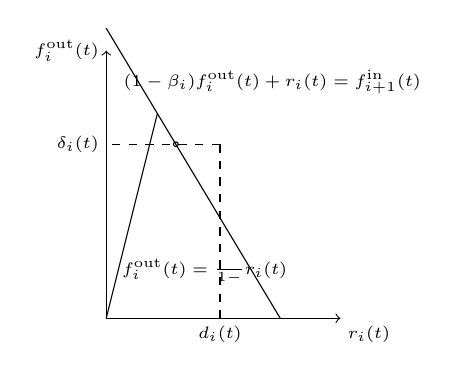
\begin{tikzpicture}[scale=1*.85,domain=0:1]

\def \rampDem{1.7}
\def \dem{2.6}
\def \priorityRat{0.8}
\def \splitRat{0.4}
\def \totalFlow{2.6}
\FontSmall

\coordinate (Z) at (0,0);
\coordinate (I1) at (\rampDem, 0);
\coordinate (I2) at (0, \dem);
\coordinate (I3) at (\rampDem, \dem);

\coordinate (A) at (0, {\totalFlow/(1-\splitRat)});
\coordinate (B) at (\totalFlow, 0);
\coordinate (C) at ({(1-\priorityRat)/\priorityRat*\dem}, \dem);
\coordinate (D) at (intersection of A--B and Z--C);


\draw[->] (Z) -- (3.5,0) node[below right]{$r_i(t)$};
\draw[->] (Z) -- (0,4) node[left]{$f^{\text{out}}_i(t)$};

\draw[dashed] (I3) -- (I1) node[below]{$d_i(t)$};
\draw[dashed] (I3) -- (I2) node[left]{$\delta_i(t)$};


\begin{scope}
%\clip (Z) rectangle (3.5,4);
\draw (A) -- (B) node[yshift=3cm, xshift=-0.1cm]{$(1-\beta_i)f_i^{\text{out}}(t) + r_i(t) = f_{i+1}^{\text{in}}(t)$};
\end{scope}

\draw (Z) -- (D) node[yshift=-2cm, xshift=0.6cm]{$f_i^{\text{out}}(t) = \frac{\priority{\icell}}{1-\priority{\icell}} r_i(t)$};
\draw (intersection of A--B and I3--I2) circle (1pt);

\end{tikzpicture}
}
\label{fig:junctionBuffer-junctionFlowsInside}
\end{figure}
\end{minipage}\hfill
\begin{minipage}[t]{0.50\linewidth}
\begin{align}
&& \flowin{\icell+1}{\itime} & =  \underbrace{\rampflow{\icell}{\itime}}_{=(1-P)\flowin{\icell+1}{\itime}} + \underbrace{\flowout{\icell}{\itime}\left(1-\offrampratio{\icell}{\itime}\right)}_{=P\flowin{\icell+1}{\itime}}& \nonumber
\end{align}
\pause \begin{align}
&& \flowout{\icell}{\itime} &= \celldemand{\icell}{\itime} \nonumber \\
&& &\text{if } \priority{\icell}\flowin{\icell+1}{\itime} > \left(1-\offrampratio{\icell}{\itime}\right)\celldemand{\icell}{\itime} \nonumber
\end{align}
\end{minipage}




\end{frame}

%-----------------------------------------------------------------------------------------------------------------------------------------------------------------
\begin{frame}{Junction inflow}

\Fontvi

\begin{figure}[t]
\hspace{\systemDiagOffset}
\resizebox{\systemDiagResizeMult\columnwidth}{!}{%indices
\global\long\def\itime{k}
\global\long\def\icell{i}
\global\long\def\iconst{h}

\global\long\def\ntime{T}
\global\long\def\ncell{N}
\global\long\def\nconst{8}

%constants
\global\long\def\deltat{\triangle t}
\global\long\def\deltax{\triangle x}


\global\long\def\prioritysymbol{P}
 \global\long\def\priority#1{\prioritysymbol_{#1}}


%ramps
\global\long\def\rampcontrolsymbol{u}
 \global\long\def\rampcontrol#1#2{\rampcontrolsymbol_{#1}\left(#2\right)}
 \global\long\def\rampcontrolMax#1{\rampcontrolsymbol_{#1}^{\max}}
 \global\long\def\rampqueuesymbol{l}
 \global\long\def\rampqueue#1#2{\rampqueuesymbol_{#1}\left(#2\right)}
 \global\long\def\rampqueueinit#1{\rampqueuesymbol_{#1}^{0}}
 \global\long\def\rampflowsymbol{r}
 \global\long\def\rampflow#1#2{\rampflowsymbol_{#1}\left(#2\right)}


\global\long\def\offrampratiosymbol{\beta}
 \global\long\def\offrampratio#1#2{\offrampratiosymbol_{#1}\left(#2\right)}


%cells
\global\long\def\flowsymbol{f}
 \global\long\def\flowout#1#2{\flowsymbol_{#1}^{\text{out}}\left(#2\right)}
 \global\long\def\flowin#1#2{\flowsymbol_{#1}^{\text{in}}\left(#2\right)}
 

\global\long\def\densitysymbol{\rho}
 \global\long\def\density#1#2{\densitysymbol_{#1}\left(#2\right)}
 \global\long\def\densityinit#1{\densitysymbol_{#1}^{0}}


%input
\global\long\def\inputfluxsymbol{D}
 \global\long\def\inputflux#1#2{D_{#1}\left(#2\right)}


%supply and demand
\global\long\def\celldemandsymbol{\delta}
 \global\long\def\celldemand#1#2{\celldemandsymbol_{#1}\left(#2\right)}


\global\long\def\cellsupplysymbol{\sigma}
 \global\long\def\cellsupply#1#2{\cellsupplysymbol_{#1}\left(#2\right)}


\global\long\def\rampdemandsymbol{d}
 \global\long\def\rampdemand#1#2{\rampdemandsymbol_{#1}\left(#2\right)}


%parameters
\global\long\def\ffspeedsymbol{v}
 \global\long\def\ffspeed#1{\ffspeedsymbol_{#1}}


\global\long\def\congspeedsymbol{w}
 \global\long\def\congspeed#1{\congspeedsymbol_{#1}}


\global\long\def\fmaxsymbol{F}
 \global\long\def\fmax#1{\fmaxsymbol_{#1}}


\global\long\def\jamdensitysymbol{\densitysymbol^{\text{jam}}}
 \global\long\def\jamdensity#1{\jamdensitysymbol_{#1}}


%adjoint
\global\long\def\state#1#2{x_{#1}\left( #2 \right)}
\global\long\def\ind#1{1_{\left\{#1\right\}}}

\global\long\def\stdidx#1{#1{\itime}{\icell}}
\global\long\def\sstdidx#1{\stdidx{#1{\iconst}}}

\global\long\def\H#1#2#3{H^{#1}_{#2, #3}}
\global\long\def\stdH#1{\stdidx{\H{#1}}}
\global\long\def\sstdH{\sstdidx{\H}}

\global\long\def\G#1#2#3{G^{#1}_{#2, #3}}
\global\long\def\stdG#1{\stdidx{\G{#1}}}
\global\long\def\sstdG{\sstdidx{\G}}

\global\long\def\Lambd#1#2#3{\lambda^{#1}_{#2, #3}}
\global\long\def\stdLambd#1{\stdidx{\Lambd{#1}}}
\global\long\def\sstdLambd{\sstdidx{\Lambd}}

% \global\long\def\R#1#2#3{R{#1}_{#2, #3}}

% Riemann problem
\global\long\def\rs{\mathcal{RS}}
\global\long\def\js{\mathcal{JS}}



\begin{tikzpicture}[scale=1.4]

\def \linkWidth {1cm}
\def \nodeWidth {0.3cm}

\coordinate (arrow) at (1.8,0);
\coordinate (dots) at (0.5,0);
\coordinate (unit) at (2.5,0);

%\node (link0) at (0,0) [rectangle, minimum width=\linkWidth, draw] {$0$};
%\node (link1) at ($(link0) + 1*(unit)$) [rectangle, minimum width=\linkWidth, draw] {$1$};
\node (linkI) at (-2,0) [rectangle, minimum width=\linkWidth, draw] {$\icell$};
\node (nodeI) at ($(linkI) + 1*(unit)$) [circle, minimum width=\nodeWidth, draw] {$\icell$};

\node (onrampI) at ($(linkI)-(0,0.8)$) [rectangle, minimum width=\linkWidth, draw] {on-ramp $\icell$};
\node (offrampI) at ($(linkI) + 1.4*(unit) - (0,0.5)$) {};

\node (linkI1) at ($(nodeI) + 1.45*(unit)$) [rectangle, minimum width=\linkWidth, draw] {$\icell+1$};

%\node (linkN) at ($(linkI1)+1.8*(unit)$) [rectangle, minimum width=\linkWidth, draw] {$\ncell$};

% link 0
%\draw[->] ($(link0)-(arrow)$) -- (link0) node[above, midway] {$\inputflux{0}{\itime}$};
%\draw[->] (link0) -- (link1) node[above, midway] {$\flowout{0}{\itime}$};

% link 1
%\draw[->] (link1) -- ($(link1) + (arrow)$) node[above, midway] {$\flowout{1}{\itime}$};

%dots
%\draw ($(link1) + (arrow) + (dots)$) node{$\dots$} ;

% link i
\draw[->] ($(linkI) - 1.3*(arrow)$) -- (linkI)node[above, xshift=-1.1cm] {$\flowin{\icell}{\itime}$};
\draw[->] (linkI) -- (nodeI) node[above, midway] {$\flowout{\icell}{\itime}$};
\draw[->] (nodeI) -- (linkI1) node[above, xshift=-1.1cm]{$\flowin{\icell+1}{\itime}$} ;

%node i
\draw[->] (onrampI) [anchor=right]-- (nodeI) node[below, midway]{$\rampflow{\icell}{\itime}$};
\draw[->] ($(onrampI) - (arrow)$) [anchor=right]-- (onrampI) node[above, midway]{$\inputflux{\icell}{\itime}$};
\draw[->] (nodeI) -- (offrampI) node[below, xshift=-0.3cm]{$\offrampratio{\icell}{\itime} \flowout{\icell}{\itime}$};

%link i+1
\draw[->] (linkI1) -- ($(linkI1) + (arrow)$) node[above, midway] {$\flowout{\icell+1}{\itime}$};

%dots
\draw ($(linkI1)+(arrow)+(dots)$) node{$\dots$} ;

% link N
%\draw[->] ($(linkN) - (arrow)$) -- (linkN) node[above, midway] {$\flowin{\ncell}{\itime}$};
%\draw[->] (linkN)--($(linkN) + (arrow)$) node[above, midway] {$\flowout{\ncell}{\itime}$};

% box
\draw[dashed] ($(linkI) + (-2,1)$) rectangle ($(nodeI) + (1.8,-1.5)$) node[below]{block $\icell$};

\end{tikzpicture}
}
\label{fig:system}
\end{figure}

\begin{minipage}[t]{0.46\linewidth}
\begin{figure}[h]
\centering
\resizebox{0.8\columnwidth}{!}{
	
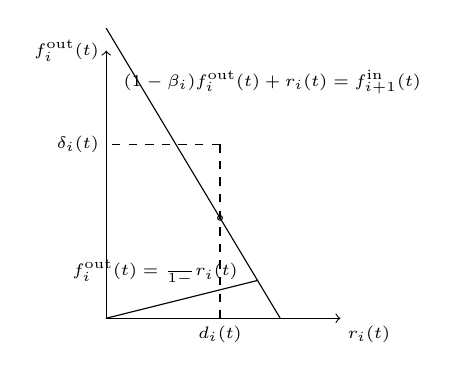
\begin{tikzpicture}[scale=1*.85,domain=0:1]

\def \rampDem{1.7}
\def \dem{2.6}
\def \priorityRat{0.2}
\def \splitRat{0.4}
\def \totalFlow{2.6}
\FontSmall

\coordinate (Z) at (0,0);
\coordinate (I1) at (\rampDem, 0);
\coordinate (I2) at (0, \dem);
\coordinate (I3) at (\rampDem, \dem);

\coordinate (A) at (0, {\totalFlow/(1-\splitRat)});
\coordinate (B) at (\totalFlow, 0);
\coordinate (C) at ({(1-\priorityRat)/\priorityRat*\dem}, \dem);
\coordinate (D) at (intersection of A--B and Z--C);


\draw[->] (Z) -- (3.5,0) node[below right]{$r_i(t)$};
\draw[->] (Z) -- (0,4) node[left]{$f^{\text{out}}_i(t)$};

\draw[dashed] (I3) -- (I1) node[below]{$d_i(t)$};
\draw[dashed] (I3) -- (I2) node[left]{$\delta_i(t)$};


\begin{scope}
%\clip (Z) rectangle (3.5,4);
\draw (A) -- (B) node[yshift=3cm, xshift=-0.1cm]{$(1-\beta_i)f_i^{\text{out}}(t) + r_i(t) = f_{i+1}^{\text{in}}(t)$};
\end{scope}

\draw (Z) -- (D) node[yshift=0.1cm, xshift=-1.3cm]{$f_i^{\text{out}}(t) = \frac{\priority{\icell}}{1-\priority{\icell}} r_i(t)$};
\draw (intersection of A--B and I3--I1) circle (1pt);

\end{tikzpicture}
}
\label{fig:junctionBuffer-junctionFlowsInside}
\end{figure}
\end{minipage}\hfill
\begin{minipage}[t]{0.50\linewidth}
\begin{align}
&& \flowin{\icell+1}{\itime} & =  \underbrace{\rampflow{\icell}{\itime}}_{=(1-P)\flowin{\icell+1}{\itime}} + \underbrace{\flowout{\icell}{\itime}\left(1-\offrampratio{\icell}{\itime}\right)}_{=P\flowin{\icell+1}{\itime}}& \nonumber
\end{align}
\pause \begin{align}
&& \flowout{\icell}{\itime} &= \frac{\flowin{\icell+1}{\itime}-\rampdemand{\icell}{\itime}}{1-\offrampratio{\icell}{\itime}} \nonumber \\
&& &\text{if } \left(1-\priority{\icell}\right)\flowin{\icell+1}{\itime} > \rampdemand{\icell}{\itime} \nonumber
\end{align}
\end{minipage}
\end{frame}

%-----------------------------------------------------------------------------------------------------------------------------------------------------------------
\begin{frame}{Junction inflow}

\Fontvi

\begin{figure}[t]
\hspace{\systemDiagOffset}
\resizebox{\systemDiagResizeMult\columnwidth}{!}{%indices
\global\long\def\itime{k}
\global\long\def\icell{i}
\global\long\def\iconst{h}

\global\long\def\ntime{T}
\global\long\def\ncell{N}
\global\long\def\nconst{8}

%constants
\global\long\def\deltat{\triangle t}
\global\long\def\deltax{\triangle x}


\global\long\def\prioritysymbol{P}
 \global\long\def\priority#1{\prioritysymbol_{#1}}


%ramps
\global\long\def\rampcontrolsymbol{u}
 \global\long\def\rampcontrol#1#2{\rampcontrolsymbol_{#1}\left(#2\right)}
 \global\long\def\rampcontrolMax#1{\rampcontrolsymbol_{#1}^{\max}}
 \global\long\def\rampqueuesymbol{l}
 \global\long\def\rampqueue#1#2{\rampqueuesymbol_{#1}\left(#2\right)}
 \global\long\def\rampqueueinit#1{\rampqueuesymbol_{#1}^{0}}
 \global\long\def\rampflowsymbol{r}
 \global\long\def\rampflow#1#2{\rampflowsymbol_{#1}\left(#2\right)}


\global\long\def\offrampratiosymbol{\beta}
 \global\long\def\offrampratio#1#2{\offrampratiosymbol_{#1}\left(#2\right)}


%cells
\global\long\def\flowsymbol{f}
 \global\long\def\flowout#1#2{\flowsymbol_{#1}^{\text{out}}\left(#2\right)}
 \global\long\def\flowin#1#2{\flowsymbol_{#1}^{\text{in}}\left(#2\right)}
 

\global\long\def\densitysymbol{\rho}
 \global\long\def\density#1#2{\densitysymbol_{#1}\left(#2\right)}
 \global\long\def\densityinit#1{\densitysymbol_{#1}^{0}}


%input
\global\long\def\inputfluxsymbol{D}
 \global\long\def\inputflux#1#2{D_{#1}\left(#2\right)}


%supply and demand
\global\long\def\celldemandsymbol{\delta}
 \global\long\def\celldemand#1#2{\celldemandsymbol_{#1}\left(#2\right)}


\global\long\def\cellsupplysymbol{\sigma}
 \global\long\def\cellsupply#1#2{\cellsupplysymbol_{#1}\left(#2\right)}


\global\long\def\rampdemandsymbol{d}
 \global\long\def\rampdemand#1#2{\rampdemandsymbol_{#1}\left(#2\right)}


%parameters
\global\long\def\ffspeedsymbol{v}
 \global\long\def\ffspeed#1{\ffspeedsymbol_{#1}}


\global\long\def\congspeedsymbol{w}
 \global\long\def\congspeed#1{\congspeedsymbol_{#1}}


\global\long\def\fmaxsymbol{F}
 \global\long\def\fmax#1{\fmaxsymbol_{#1}}


\global\long\def\jamdensitysymbol{\densitysymbol^{\text{jam}}}
 \global\long\def\jamdensity#1{\jamdensitysymbol_{#1}}


%adjoint
\global\long\def\state#1#2{x_{#1}\left( #2 \right)}
\global\long\def\ind#1{1_{\left\{#1\right\}}}

\global\long\def\stdidx#1{#1{\itime}{\icell}}
\global\long\def\sstdidx#1{\stdidx{#1{\iconst}}}

\global\long\def\H#1#2#3{H^{#1}_{#2, #3}}
\global\long\def\stdH#1{\stdidx{\H{#1}}}
\global\long\def\sstdH{\sstdidx{\H}}

\global\long\def\G#1#2#3{G^{#1}_{#2, #3}}
\global\long\def\stdG#1{\stdidx{\G{#1}}}
\global\long\def\sstdG{\sstdidx{\G}}

\global\long\def\Lambd#1#2#3{\lambda^{#1}_{#2, #3}}
\global\long\def\stdLambd#1{\stdidx{\Lambd{#1}}}
\global\long\def\sstdLambd{\sstdidx{\Lambd}}

% \global\long\def\R#1#2#3{R{#1}_{#2, #3}}

% Riemann problem
\global\long\def\rs{\mathcal{RS}}
\global\long\def\js{\mathcal{JS}}



\begin{tikzpicture}[scale=1.4]

\def \linkWidth {1cm}
\def \nodeWidth {0.3cm}

\coordinate (arrow) at (1.8,0);
\coordinate (dots) at (0.5,0);
\coordinate (unit) at (2.5,0);

%\node (link0) at (0,0) [rectangle, minimum width=\linkWidth, draw] {$0$};
%\node (link1) at ($(link0) + 1*(unit)$) [rectangle, minimum width=\linkWidth, draw] {$1$};
\node (linkI) at (-2,0) [rectangle, minimum width=\linkWidth, draw] {$\icell$};
\node (nodeI) at ($(linkI) + 1*(unit)$) [circle, minimum width=\nodeWidth, draw] {$\icell$};

\node (onrampI) at ($(linkI)-(0,0.8)$) [rectangle, minimum width=\linkWidth, draw] {on-ramp $\icell$};
\node (offrampI) at ($(linkI) + 1.4*(unit) - (0,0.5)$) {};

\node (linkI1) at ($(nodeI) + 1.45*(unit)$) [rectangle, minimum width=\linkWidth, draw] {$\icell+1$};

%\node (linkN) at ($(linkI1)+1.8*(unit)$) [rectangle, minimum width=\linkWidth, draw] {$\ncell$};

% link 0
%\draw[->] ($(link0)-(arrow)$) -- (link0) node[above, midway] {$\inputflux{0}{\itime}$};
%\draw[->] (link0) -- (link1) node[above, midway] {$\flowout{0}{\itime}$};

% link 1
%\draw[->] (link1) -- ($(link1) + (arrow)$) node[above, midway] {$\flowout{1}{\itime}$};

%dots
%\draw ($(link1) + (arrow) + (dots)$) node{$\dots$} ;

% link i
\draw[->] ($(linkI) - 1.3*(arrow)$) -- (linkI)node[above, xshift=-1.1cm] {$\flowin{\icell}{\itime}$};
\draw[->] (linkI) -- (nodeI) node[above, midway] {$\flowout{\icell}{\itime}$};
\draw[->] (nodeI) -- (linkI1) node[above, xshift=-1.1cm]{$\flowin{\icell+1}{\itime}$} ;

%node i
\draw[->] (onrampI) [anchor=right]-- (nodeI) node[below, midway]{$\rampflow{\icell}{\itime}$};
\draw[->] ($(onrampI) - (arrow)$) [anchor=right]-- (onrampI) node[above, midway]{$\inputflux{\icell}{\itime}$};
\draw[->] (nodeI) -- (offrampI) node[below, xshift=-0.3cm]{$\offrampratio{\icell}{\itime} \flowout{\icell}{\itime}$};

%link i+1
\draw[->] (linkI1) -- ($(linkI1) + (arrow)$) node[above, midway] {$\flowout{\icell+1}{\itime}$};

%dots
\draw ($(linkI1)+(arrow)+(dots)$) node{$\dots$} ;

% link N
%\draw[->] ($(linkN) - (arrow)$) -- (linkN) node[above, midway] {$\flowin{\ncell}{\itime}$};
%\draw[->] (linkN)--($(linkN) + (arrow)$) node[above, midway] {$\flowout{\ncell}{\itime}$};

% box
\draw[dashed] ($(linkI) + (-2,1)$) rectangle ($(nodeI) + (1.8,-1.5)$) node[below]{block $\icell$};

\end{tikzpicture}
}
\label{fig:system}
\end{figure}

\begin{minipage}[t]{0.46\linewidth}
\begin{figure}[h]
\centering
\resizebox{0.8\columnwidth}{!}{
	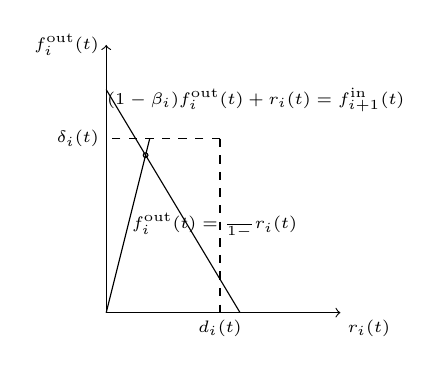
\begin{tikzpicture}[scale=1*.85,domain=0:1]

\def \rampDem{1.7}
\def \dem{2.6}
\def \priorityRat{0.8}
\def \splitRat{0.4}
\def \totalFlow{2}
\FontSmall


\coordinate (Z) at (0,0);
\coordinate (I1) at (\rampDem, 0);
\coordinate (I2) at (0, \dem);
\coordinate (I3) at (\rampDem, \dem);
\coordinate (A) at (0, {\totalFlow/(1-\splitRat)});
\coordinate (B) at (\totalFlow, 0);
\coordinate (C) at ({(1-\priorityRat)/\priorityRat*\dem}, \dem);

\draw[->] (Z) -- (3.5,0) node[below right]{$r_i(t)$};
\draw[->] (Z) -- (0,4) node[left]{$f^{\text{out}}_i(t)$};
\draw[dashed] (I3) -- (I1) node[below]{$d_i(t)$};
\draw[dashed] (I3) -- (I2) node[left]{$\delta_i(t)$};
\draw (A) -- (B) node[yshift=2.7cm, xshift=0.2cm]{$(1-\beta_i)f_i^{\text{out}}(t) + r_i(t) = f_{i+1}^{\text{in}}(t)$};
\draw (Z) -- (C) node[midway, xshift=1.1cm]{$f_i^{\text{out}}(t) = \frac{\priority{\icell}}{1-\priority{\icell}} r_i(t)$};
\draw (intersection of A--B and Z--C) circle (1pt);

\end{tikzpicture}
}
\label{fig:junctionBuffer-junctionFlows}
\end{figure}
\end{minipage}\hfill
\begin{minipage}[t]{0.50\linewidth}
\begin{align}
&& \flowin{\icell+1}{\itime} & =  \underbrace{\rampflow{\icell}{\itime}}_{=(1-P)\flowin{\icell+1}{\itime}} + \underbrace{\flowout{\icell}{\itime}\left(1-\offrampratio{\icell}{\itime}\right)}_{=P\flowin{\icell+1}{\itime}}& \nonumber 
\end{align}
\pause \begin{align}
&& \flowout{\icell}{\itime} &= \frac{\priority{\icell}\flowin{\icell+1}{\itime}}{1-\offrampratio{\icell}{\itime}} \ \ \text{otherwise }\nonumber 
\end{align}
\end{minipage}

\end{frame}

%-----------------------------------------------------------------------------------------------------------------------------------------------------------------
\begin{frame}{Junction inflow}

\Fontvi

\begin{figure}[t]
\hspace{\systemDiagOffset}
\resizebox{\systemDiagResizeMult\columnwidth}{!}{%indices
\global\long\def\itime{k}
\global\long\def\icell{i}
\global\long\def\iconst{h}

\global\long\def\ntime{T}
\global\long\def\ncell{N}
\global\long\def\nconst{8}

%constants
\global\long\def\deltat{\triangle t}
\global\long\def\deltax{\triangle x}


\global\long\def\prioritysymbol{P}
 \global\long\def\priority#1{\prioritysymbol_{#1}}


%ramps
\global\long\def\rampcontrolsymbol{u}
 \global\long\def\rampcontrol#1#2{\rampcontrolsymbol_{#1}\left(#2\right)}
 \global\long\def\rampcontrolMax#1{\rampcontrolsymbol_{#1}^{\max}}
 \global\long\def\rampqueuesymbol{l}
 \global\long\def\rampqueue#1#2{\rampqueuesymbol_{#1}\left(#2\right)}
 \global\long\def\rampqueueinit#1{\rampqueuesymbol_{#1}^{0}}
 \global\long\def\rampflowsymbol{r}
 \global\long\def\rampflow#1#2{\rampflowsymbol_{#1}\left(#2\right)}


\global\long\def\offrampratiosymbol{\beta}
 \global\long\def\offrampratio#1#2{\offrampratiosymbol_{#1}\left(#2\right)}


%cells
\global\long\def\flowsymbol{f}
 \global\long\def\flowout#1#2{\flowsymbol_{#1}^{\text{out}}\left(#2\right)}
 \global\long\def\flowin#1#2{\flowsymbol_{#1}^{\text{in}}\left(#2\right)}
 

\global\long\def\densitysymbol{\rho}
 \global\long\def\density#1#2{\densitysymbol_{#1}\left(#2\right)}
 \global\long\def\densityinit#1{\densitysymbol_{#1}^{0}}


%input
\global\long\def\inputfluxsymbol{D}
 \global\long\def\inputflux#1#2{D_{#1}\left(#2\right)}


%supply and demand
\global\long\def\celldemandsymbol{\delta}
 \global\long\def\celldemand#1#2{\celldemandsymbol_{#1}\left(#2\right)}


\global\long\def\cellsupplysymbol{\sigma}
 \global\long\def\cellsupply#1#2{\cellsupplysymbol_{#1}\left(#2\right)}


\global\long\def\rampdemandsymbol{d}
 \global\long\def\rampdemand#1#2{\rampdemandsymbol_{#1}\left(#2\right)}


%parameters
\global\long\def\ffspeedsymbol{v}
 \global\long\def\ffspeed#1{\ffspeedsymbol_{#1}}


\global\long\def\congspeedsymbol{w}
 \global\long\def\congspeed#1{\congspeedsymbol_{#1}}


\global\long\def\fmaxsymbol{F}
 \global\long\def\fmax#1{\fmaxsymbol_{#1}}


\global\long\def\jamdensitysymbol{\densitysymbol^{\text{jam}}}
 \global\long\def\jamdensity#1{\jamdensitysymbol_{#1}}


%adjoint
\global\long\def\state#1#2{x_{#1}\left( #2 \right)}
\global\long\def\ind#1{1_{\left\{#1\right\}}}

\global\long\def\stdidx#1{#1{\itime}{\icell}}
\global\long\def\sstdidx#1{\stdidx{#1{\iconst}}}

\global\long\def\H#1#2#3{H^{#1}_{#2, #3}}
\global\long\def\stdH#1{\stdidx{\H{#1}}}
\global\long\def\sstdH{\sstdidx{\H}}

\global\long\def\G#1#2#3{G^{#1}_{#2, #3}}
\global\long\def\stdG#1{\stdidx{\G{#1}}}
\global\long\def\sstdG{\sstdidx{\G}}

\global\long\def\Lambd#1#2#3{\lambda^{#1}_{#2, #3}}
\global\long\def\stdLambd#1{\stdidx{\Lambd{#1}}}
\global\long\def\sstdLambd{\sstdidx{\Lambd}}

% \global\long\def\R#1#2#3{R{#1}_{#2, #3}}

% Riemann problem
\global\long\def\rs{\mathcal{RS}}
\global\long\def\js{\mathcal{JS}}



\begin{tikzpicture}[scale=1.4]

\def \linkWidth {1cm}
\def \nodeWidth {0.3cm}

\coordinate (arrow) at (1.8,0);
\coordinate (dots) at (0.5,0);
\coordinate (unit) at (2.5,0);

%\node (link0) at (0,0) [rectangle, minimum width=\linkWidth, draw] {$0$};
%\node (link1) at ($(link0) + 1*(unit)$) [rectangle, minimum width=\linkWidth, draw] {$1$};
\node (linkI) at (-2,0) [rectangle, minimum width=\linkWidth, draw] {$\icell$};
\node (nodeI) at ($(linkI) + 1*(unit)$) [circle, minimum width=\nodeWidth, draw] {$\icell$};

\node (onrampI) at ($(linkI)-(0,0.8)$) [rectangle, minimum width=\linkWidth, draw] {on-ramp $\icell$};
\node (offrampI) at ($(linkI) + 1.4*(unit) - (0,0.5)$) {};

\node (linkI1) at ($(nodeI) + 1.45*(unit)$) [rectangle, minimum width=\linkWidth, draw] {$\icell+1$};

%\node (linkN) at ($(linkI1)+1.8*(unit)$) [rectangle, minimum width=\linkWidth, draw] {$\ncell$};

% link 0
%\draw[->] ($(link0)-(arrow)$) -- (link0) node[above, midway] {$\inputflux{0}{\itime}$};
%\draw[->] (link0) -- (link1) node[above, midway] {$\flowout{0}{\itime}$};

% link 1
%\draw[->] (link1) -- ($(link1) + (arrow)$) node[above, midway] {$\flowout{1}{\itime}$};

%dots
%\draw ($(link1) + (arrow) + (dots)$) node{$\dots$} ;

% link i
\draw[->] ($(linkI) - 1.3*(arrow)$) -- (linkI)node[above, xshift=-1.1cm] {$\flowin{\icell}{\itime}$};
\draw[->] (linkI) -- (nodeI) node[above, midway] {$\flowout{\icell}{\itime}$};
\draw[->] (nodeI) -- (linkI1) node[above, xshift=-1.1cm]{$\flowin{\icell+1}{\itime}$} ;

%node i
\draw[->] (onrampI) [anchor=right]-- (nodeI) node[below, midway]{$\rampflow{\icell}{\itime}$};
\draw[->] ($(onrampI) - (arrow)$) [anchor=right]-- (onrampI) node[above, midway]{$\inputflux{\icell}{\itime}$};
\draw[->] (nodeI) -- (offrampI) node[below, xshift=-0.3cm]{$\offrampratio{\icell}{\itime} \flowout{\icell}{\itime}$};

%link i+1
\draw[->] (linkI1) -- ($(linkI1) + (arrow)$) node[above, midway] {$\flowout{\icell+1}{\itime}$};

%dots
\draw ($(linkI1)+(arrow)+(dots)$) node{$\dots$} ;

% link N
%\draw[->] ($(linkN) - (arrow)$) -- (linkN) node[above, midway] {$\flowin{\ncell}{\itime}$};
%\draw[->] (linkN)--($(linkN) + (arrow)$) node[above, midway] {$\flowout{\ncell}{\itime}$};

% box
\draw[dashed] ($(linkI) + (-2,1)$) rectangle ($(nodeI) + (1.8,-1.5)$) node[below]{block $\icell$};

\end{tikzpicture}
}
\label{fig:system}
\end{figure}

\begin{subequations}
\begin{multline}
\flowout{\icell}{\itime}
=\begin{cases}
\celldemand{\icell}{\itime} 
& \text{if } (\R{1}{\itime}{\icell}) : \priority{\icell}\flowin{\icell+1}{\itime} > \left(1-\offrampratio{\icell}{\itime}\right)\celldemand{\icell}{\itime}
\\
\frac{\flowin{\icell+1}{\itime}-\rampdemand{\icell}{\itime}}{1-\offrampratio{\icell}{\itime}}
& \text{if } (\R{2}{\itime}{\icell}) : \left(1-\priority{\icell}\right)\flowin{\icell+1}{\itime} > \rampdemand{\icell}{\itime}
\\
\frac{\priority{\icell}\flowin{\icell+1}{\itime}}{1-\offrampratio{\icell}{\itime}} & \text{otherwise } (\R{3}{\itime}{\icell})
\end{cases} \\
\forall\icell\in\left\{ 1,\ldots,\ncell-1\right\} ,\itime\in\left\{ 0,\ldots,\ntime-1\right\}
\tag{H7a}
\label{eq:junctionPriority}
\end{multline}
\begin{align}
&& \flowout{0}{\itime} & =\flowin{1}{\itime} &
\forall \itime \in \left \{ 0, \dots, \ntime-1 \right\}
\tag{H7b}
\label{eq:junctionFlowConservationSpecial1}	
\end{align}
\end{subequations}

\end{frame}
%-----------------------------------------------------------------------------------------------------------------------------------------------------------------
\begin{frame}{Ramp flow}

\Fontvi

\begin{figure}[t]
\hspace{\systemDiagOffset}
\resizebox{\systemDiagResizeMult\columnwidth}{!}{%indices
\global\long\def\itime{k}
\global\long\def\icell{i}
\global\long\def\iconst{h}

\global\long\def\ntime{T}
\global\long\def\ncell{N}
\global\long\def\nconst{8}

%constants
\global\long\def\deltat{\triangle t}
\global\long\def\deltax{\triangle x}


\global\long\def\prioritysymbol{P}
 \global\long\def\priority#1{\prioritysymbol_{#1}}


%ramps
\global\long\def\rampcontrolsymbol{u}
 \global\long\def\rampcontrol#1#2{\rampcontrolsymbol_{#1}\left(#2\right)}
 \global\long\def\rampcontrolMax#1{\rampcontrolsymbol_{#1}^{\max}}
 \global\long\def\rampqueuesymbol{l}
 \global\long\def\rampqueue#1#2{\rampqueuesymbol_{#1}\left(#2\right)}
 \global\long\def\rampqueueinit#1{\rampqueuesymbol_{#1}^{0}}
 \global\long\def\rampflowsymbol{r}
 \global\long\def\rampflow#1#2{\rampflowsymbol_{#1}\left(#2\right)}


\global\long\def\offrampratiosymbol{\beta}
 \global\long\def\offrampratio#1#2{\offrampratiosymbol_{#1}\left(#2\right)}


%cells
\global\long\def\flowsymbol{f}
 \global\long\def\flowout#1#2{\flowsymbol_{#1}^{\text{out}}\left(#2\right)}
 \global\long\def\flowin#1#2{\flowsymbol_{#1}^{\text{in}}\left(#2\right)}
 

\global\long\def\densitysymbol{\rho}
 \global\long\def\density#1#2{\densitysymbol_{#1}\left(#2\right)}
 \global\long\def\densityinit#1{\densitysymbol_{#1}^{0}}


%input
\global\long\def\inputfluxsymbol{D}
 \global\long\def\inputflux#1#2{D_{#1}\left(#2\right)}


%supply and demand
\global\long\def\celldemandsymbol{\delta}
 \global\long\def\celldemand#1#2{\celldemandsymbol_{#1}\left(#2\right)}


\global\long\def\cellsupplysymbol{\sigma}
 \global\long\def\cellsupply#1#2{\cellsupplysymbol_{#1}\left(#2\right)}


\global\long\def\rampdemandsymbol{d}
 \global\long\def\rampdemand#1#2{\rampdemandsymbol_{#1}\left(#2\right)}


%parameters
\global\long\def\ffspeedsymbol{v}
 \global\long\def\ffspeed#1{\ffspeedsymbol_{#1}}


\global\long\def\congspeedsymbol{w}
 \global\long\def\congspeed#1{\congspeedsymbol_{#1}}


\global\long\def\fmaxsymbol{F}
 \global\long\def\fmax#1{\fmaxsymbol_{#1}}


\global\long\def\jamdensitysymbol{\densitysymbol^{\text{jam}}}
 \global\long\def\jamdensity#1{\jamdensitysymbol_{#1}}


%adjoint
\global\long\def\state#1#2{x_{#1}\left( #2 \right)}
\global\long\def\ind#1{1_{\left\{#1\right\}}}

\global\long\def\stdidx#1{#1{\itime}{\icell}}
\global\long\def\sstdidx#1{\stdidx{#1{\iconst}}}

\global\long\def\H#1#2#3{H^{#1}_{#2, #3}}
\global\long\def\stdH#1{\stdidx{\H{#1}}}
\global\long\def\sstdH{\sstdidx{\H}}

\global\long\def\G#1#2#3{G^{#1}_{#2, #3}}
\global\long\def\stdG#1{\stdidx{\G{#1}}}
\global\long\def\sstdG{\sstdidx{\G}}

\global\long\def\Lambd#1#2#3{\lambda^{#1}_{#2, #3}}
\global\long\def\stdLambd#1{\stdidx{\Lambd{#1}}}
\global\long\def\sstdLambd{\sstdidx{\Lambd}}

% \global\long\def\R#1#2#3{R{#1}_{#2, #3}}

% Riemann problem
\global\long\def\rs{\mathcal{RS}}
\global\long\def\js{\mathcal{JS}}



\begin{tikzpicture}[scale=1.4]

\def \linkWidth {1cm}
\def \nodeWidth {0.3cm}

\coordinate (arrow) at (1.8,0);
\coordinate (dots) at (0.5,0);
\coordinate (unit) at (2.5,0);

%\node (link0) at (0,0) [rectangle, minimum width=\linkWidth, draw] {$0$};
%\node (link1) at ($(link0) + 1*(unit)$) [rectangle, minimum width=\linkWidth, draw] {$1$};
\node (linkI) at (-2,0) [rectangle, minimum width=\linkWidth, draw] {$\icell$};
\node (nodeI) at ($(linkI) + 1*(unit)$) [circle, minimum width=\nodeWidth, draw] {$\icell$};

\node (onrampI) at ($(linkI)-(0,0.8)$) [rectangle, minimum width=\linkWidth, draw] {on-ramp $\icell$};
\node (offrampI) at ($(linkI) + 1.4*(unit) - (0,0.5)$) {};

\node (linkI1) at ($(nodeI) + 1.45*(unit)$) [rectangle, minimum width=\linkWidth, draw] {$\icell+1$};

%\node (linkN) at ($(linkI1)+1.8*(unit)$) [rectangle, minimum width=\linkWidth, draw] {$\ncell$};

% link 0
%\draw[->] ($(link0)-(arrow)$) -- (link0) node[above, midway] {$\inputflux{0}{\itime}$};
%\draw[->] (link0) -- (link1) node[above, midway] {$\flowout{0}{\itime}$};

% link 1
%\draw[->] (link1) -- ($(link1) + (arrow)$) node[above, midway] {$\flowout{1}{\itime}$};

%dots
%\draw ($(link1) + (arrow) + (dots)$) node{$\dots$} ;

% link i
\draw[->] ($(linkI) - 1.3*(arrow)$) -- (linkI)node[above, xshift=-1.1cm] {$\flowin{\icell}{\itime}$};
\draw[->] (linkI) -- (nodeI) node[above, midway] {$\flowout{\icell}{\itime}$};
\draw[->] (nodeI) -- (linkI1) node[above, xshift=-1.1cm]{$\flowin{\icell+1}{\itime}$} ;

%node i
\draw[->] (onrampI) [anchor=right]-- (nodeI) node[below, midway]{$\rampflow{\icell}{\itime}$};
\draw[->] ($(onrampI) - (arrow)$) [anchor=right]-- (onrampI) node[above, midway]{$\inputflux{\icell}{\itime}$};
\draw[->] (nodeI) -- (offrampI) node[below, xshift=-0.3cm]{$\offrampratio{\icell}{\itime} \flowout{\icell}{\itime}$};

%link i+1
\draw[->] (linkI1) -- ($(linkI1) + (arrow)$) node[above, midway] {$\flowout{\icell+1}{\itime}$};

%dots
\draw ($(linkI1)+(arrow)+(dots)$) node{$\dots$} ;

% link N
%\draw[->] ($(linkN) - (arrow)$) -- (linkN) node[above, midway] {$\flowin{\ncell}{\itime}$};
%\draw[->] (linkN)--($(linkN) + (arrow)$) node[above, midway] {$\flowout{\ncell}{\itime}$};

% box
\draw[dashed] ($(linkI) + (-2,1)$) rectangle ($(nodeI) + (1.8,-1.5)$) node[below]{block $\icell$};

\end{tikzpicture}
}
\label{fig:system}
\end{figure}

\begin{align}
&& \rampflow{\icell}{\itime} & = \flowin{\icell+1}{\itime} - \flowout{\icell}{\itime}\left(1-\offrampratio{\icell}{\itime}\right)& \forall\icell\in\left\{ 1,\ldots,\ncell-1\right\} ,\itime\in\left\{ 0,\ldots,\ntime-1\right\}
\tag{H8}
\label{eq:junctionFlowConservation}
\end{align}

\end{frame}

%-----------------------------------------------------------------------------------------------------------------------------------------------------------------
\subsection{Lower triangular forward system}
\begin{frame}{Lower triangular forward system}

The forward system $H$ has $C$ constraints that need to be satisfied over $T$ time steps for $N$ cells.
\newline

\begin{enumerate}
\item The causality of the system implies that the state at time $t$ only depends on the state at times $t' \leq t$, so we first iterate over time.
\item At each time step, the nature of our system also allows a topological ordering of the variables (no loops in the dependency graph!)
\item Finally we iterate over the cells, as there is no equation that couples the same variable at a given time step for two seperate cells. 
\end{enumerate}

%The dimension of $\frac{\partial H}{\partial x}$ is $T \cdot C \cdot N \times T \cdot X \cdot N$

\end{frame}

%-----------------------------------------------------------------------------------------------------------------------------------------------------------------
\begin{frame}{Lower triangular forward system}

\begin{figure}[h]
\hspace{-40.2in}
\resizebox{44in}{!}{
%% =================
% layers
%% =================

\pgfdeclarelayer{timelayer}
\pgfdeclarelayer{varlayer}
\pgfdeclarelayer{celllayer}
\pgfsetlayers{timelayer,varlayer,celllayer}


%% =================
% absolute constants
%% =================


\def\clscellsize{4.5}
\def\blockdist{2.3}
\def\edgedist{2.5}
\def\clsdist{.1}
\def\varmargin{.25}
\def\timemargin{.25}

%% =================
% relative constants
%% =================


\def\clsgrpdist{\clscellsize * .1}
\def\vargrpdist{\clscellsize * .4}
\def\timegrpdist{\clscellsize * 1.5}


%% =================
% styles
%% =================


\tikzstyle{clsnode} = [draw, fill = white, shape = circle, minimum height=\clscellsize em]
\tikzstyle{varnode} = [draw, fill = yellow!10]
\tikzstyle{timenode} = [draw, fill = blue!10]
\tikzstyle{myarrow} = [draw, ->, line width = 2]


\begin{tikzpicture}
%% =================
% time step 0
%% =================


%% =================
% densities
%% =================

    \begin{pgfonlayer}{celllayer}
        \node (rho1) [clsnode] {$\density{0}{0}$};
        \path (rho1.north)+(0,\clsdist) node (rho2) [clsnode] {$\cdots$};
        \path (rho2.north)+(0,\clsdist) node (rho3) [clsnode] {$\density{\ncell}{0}$};

        \path (rho1.east)+(\clsgrpdist,0) node (l1) [clsnode] {$\rampqueue{1}{0}$};
        \path (l1.north)+(0,\clsdist) node (l2) [clsnode] {$\cdots$};
        \path (l2.north)+(0,\clsdist) node (l3) [clsnode] {$\rampqueue{\ncell-1}{0}$};
    \end{pgfonlayer}

%% =================
% densities box
%% =================

    \begin{pgfonlayer}{varlayer}
        \path (rho3.west |- rho3.north)+(-\varmargin,\varmargin) node (tlvar1) {};
        \path (l1.east |- l1.south)+(\varmargin,-\varmargin) node (brvar1) {};
        \path [varnode] (tlvar1) rectangle (brvar1);
    \end{pgfonlayer}

%% =================
% demands
%% =================


    \begin{pgfonlayer}{celllayer}
        \path (l1.east)+(\vargrpdist,0) node (del1) [clsnode] {$\celldemand{0}{0}$};
        \path (del1.north)+(0,\clsdist) node (del2) [clsnode] {$\cdots$};
        \path (del2.north)+(0,\clsdist) node (del3) [clsnode] {$\celldemand{\ncell}{0}$};

        \path (del1.east)+(\clsgrpdist,0) node (sig1) [clsnode] {$\cellsupply{1}{0}$};
        \path (sig1.north)+(0,\clsdist) node (sig2) [clsnode] {$\cdots$};
        \path (sig2.north)+(0,\clsdist) node (sig3) [clsnode] {$\cellsupply{\ncell}{0}$};

        \path (sig1.east)+(\clsgrpdist,0) node (d1) [clsnode] {$d_{1}(0)$};
        \path (d1.north)+(0,\clsdist) node (d2) [clsnode] {$\cdots$};
        \path (d2.north)+(0,\clsdist) node (d3) [clsnode] {$d_{\ncell}(0)$};
    \end{pgfonlayer}
    \begin{pgfonlayer}{varlayer}
        \path (del3.west |- del3.north)+(-\varmargin,\varmargin) node (tlvar2) {};
        \path (d1.east |- d1.south)+(\varmargin,-\varmargin) node (brvar2) {};
        \path [varnode] (tlvar2) rectangle (brvar2);
        \path [myarrow] (l2.east -| brvar1) -- (del2.west -| tlvar2);
    \end{pgfonlayer}

%% =================
% flow ins
%% =================


    \begin{pgfonlayer}{celllayer}
        \path (d1.east)+(\vargrpdist,0) node (fin1) [clsnode] {$\flowin{1}{0}$};
        \path (fin1.north)+(0,\clsdist) node (fin2) [clsnode] {$\cdots$};
        \path (fin2.north)+(0,\clsdist) node (fin3) [clsnode] {$\flowin{\ncell}{0}$};
    \end{pgfonlayer}
    \begin{pgfonlayer}{varlayer}
        \path (fin3.west |- fin3.north)+(-\varmargin,\varmargin) node (tlvar3) {};
        \path (fin1.east |- fin1.south)+(\varmargin,-\varmargin) node (brvar3) {};
        \path [varnode] (tlvar3) rectangle (brvar3);
        \path [myarrow] (d2.east -| brvar2) -- (tlvar3 |- fin2.west);
    \end{pgfonlayer}

%% =================
% flow outs
%% =================

    \begin{pgfonlayer}{celllayer}
        \path (fin1.east)+(\vargrpdist,0) node (fout1) [clsnode] {$\flowout{1}{0}$};
        \path (fout1.north)+(0,\clsdist) node (fout2) [clsnode] {$\cdots$};
        \path (fout2.north)+(0,\clsdist) node (fout3) [clsnode] {$\flowout{\ncell-1}{0}$};
    \end{pgfonlayer}
    \begin{pgfonlayer}{varlayer}
        \path (fout3.west |- fout3.north)+(-\varmargin,\varmargin) node (tlvar4) {};
        \path (fout1.east |- fout1.south)+(\varmargin,-\varmargin) node (brvar4) {};
        \path [varnode] (tlvar4) rectangle (brvar4);
        \path [myarrow] (fin2.east -| brvar3) -- (tlvar4 |- fout2.west);
    \end{pgfonlayer}

%% =================
% ramps
%% =================

    \begin{pgfonlayer}{celllayer}
        \path (fout1.east)+(\vargrpdist,0) node (r1) [clsnode] {$\rampflow{1}{0}$};
        \path (r1.north)+(0,\clsdist) node (r2) [clsnode] {$\cdots$};
        \path (r2.north)+(0,\clsdist) node (r3) [clsnode] {$\rampflow{\ncell-1}{0}$};
    \end{pgfonlayer}
    \begin{pgfonlayer}{varlayer}
        \path (r3.west |- r3.north)+(-\varmargin,\varmargin) node (tlvar5) {};
        \path (r1.east |- r1.south)+(\varmargin,-\varmargin) node (brvar5) {};
        \path [varnode] (tlvar5) rectangle (brvar5);
        \path [myarrow] (fout2.east -| brvar4) -- (tlvar5 |- r2.west);
    \end{pgfonlayer}

%% =================
% time box
%% =================


    \begin{pgfonlayer}{timelayer}
        \path (tlvar1)+(-\timemargin,\timemargin) node (tltime1) {};
        \path (brvar5)+(\timemargin,-\timemargin*3) node (brtime1) {};
        \path [timenode] (tltime1) rectangle (brtime1) node (varbox) {};
        \gettikzxy{(brtime1)}{\bx}{\by};
        \gettikzxy{(tltime1)}{\tx}{\ty};
        \path [text centered] (brtime1)+(\tx*.5 - \bx*.5,.3) node (timelabel1) {Time 0};
    \end{pgfonlayer}


%% =================
% time step N
%% =================


    \begin{pgfonlayer}{celllayer}
        \path (rho1.south)+(0,-\timegrpdist) node (rho1) [clsnode] {$\density{1}{\ntime}$};
        \path (rho1.north)+(0,\clsdist) node (rho2) [clsnode] {$\cdots$};
        \path (rho2.north)+(0,\clsdist) node (rho3) [clsnode] {$\density{\ncell}{\ntime}$};

        \path (rho1.east)+(\clsgrpdist,0) node (l1) [clsnode] {$\rampqueue{1}{\ntime}$};
        \path (l1.north)+(0,\clsdist) node (l2) [clsnode] {$\cdots$};
        \path (l2.north)+(0,\clsdist) node (l3) [clsnode] {$\rampqueue{\ncell-1}{\ntime}$};
    \end{pgfonlayer}
    \begin{pgfonlayer}{varlayer}
        \path (rho3.west |- rho3.north)+(-\varmargin,\varmargin) node (tlvar1) {};
        \path (l1.east |- l1.south)+(\varmargin,-\varmargin) node (brvar1) {};
        \path [varnode] (tlvar1) rectangle (brvar1);
    \end{pgfonlayer}

    \begin{pgfonlayer}{celllayer}
        \path (l1.east)+(\vargrpdist,0) node (del1) [clsnode] {$\celldemand{0}{\ntime}$};
        \path (del1.north)+(0,\clsdist) node (del2) [clsnode] {$\cdots$};
        \path (del2.north)+(0,\clsdist) node (del3) [clsnode] {$\celldemand{\ncell}{\ntime}$};

        \path (del1.east)+(\clsgrpdist,0) node (sig1) [clsnode] {$\cellsupply{1}{\ntime}$};
        \path (sig1.north)+(0,\clsdist) node (sig2) [clsnode] {$\cdots$};
        \path (sig2.north)+(0,\clsdist) node (sig3) [clsnode] {$\cellsupply{\ncell}{\ntime}$};

        \path (sig1.east)+(\clsgrpdist,0) node (d1) [clsnode] {$d_{1}(\ntime)$};
        \path (d1.north)+(0,\clsdist) node (d2) [clsnode] {$\cdots$};
        \path (d2.north)+(0,\clsdist) node (d3) [clsnode] {$d_{\ncell}(\ntime)$};

    \end{pgfonlayer}
    \begin{pgfonlayer}{varlayer}
        \path (del3.west |- del3.north)+(-\varmargin,\varmargin) node (tlvar2) {};
        \path (d1.east |- d1.south)+(\varmargin,-\varmargin) node (brvar2) {};
        \path [varnode] (tlvar2) rectangle (brvar2);
        \path [myarrow] (l2.east -| brvar1) -- (del2.west -| tlvar2);
    \end{pgfonlayer}

    \begin{pgfonlayer}{celllayer}
        \path (d1.east)+(\vargrpdist,0) node (fin1) [clsnode] {$\flowin{1}{\ntime}$};
        \path (fin1.north)+(0,\clsdist) node (fin2) [clsnode] {$\cdots$};
        \path (fin2.north)+(0,\clsdist) node (fin3) [clsnode] {$\flowin{\ncell}{\ntime}$};
    \end{pgfonlayer}
    \begin{pgfonlayer}{varlayer}
        \path (fin3.west |- fin3.north)+(-\varmargin,\varmargin) node (tlvar3) {};
        \path (fin1.east |- fin1.south)+(\varmargin,-\varmargin) node (brvar3) {};
        \path [varnode] (tlvar3) rectangle (brvar3);
        \path [myarrow] (d2.east -| brvar2) -- (tlvar3 |- fin2.west);
    \end{pgfonlayer}


    \begin{pgfonlayer}{celllayer}
        \path (fin1.east)+(\vargrpdist,0) node (fout1) [clsnode] {$\flowout{1}{\ntime}$};
        \path (fout1.north)+(0,\clsdist) node (fout2) [clsnode] {$\cdots$};
        \path (fout2.north)+(0,\clsdist) node (fout3) [clsnode] {$\flowout{\ncell-1}{\ntime}$};
    \end{pgfonlayer}
    \begin{pgfonlayer}{varlayer}
        \path (fout3.west |- fout3.north)+(-\varmargin,\varmargin) node (tlvar4) {};
        \path (fout1.east |- fout1.south)+(\varmargin,-\varmargin) node (brvar4) {};
        \path [varnode] (tlvar4) rectangle (brvar4);
        \path [myarrow] (fin2.east -| brvar3) -- (tlvar4 |- fout2.west);
    \end{pgfonlayer}


    \begin{pgfonlayer}{celllayer}
        \path (fout1.east)+(\vargrpdist,0) node (r1) [clsnode] {$\rampflow{1}{\ntime}$};
        \path (r1.north)+(0,\clsdist) node (r2) [clsnode] {$\cdots$};
        \path (r2.north)+(0,\clsdist) node (r3) [clsnode] {$\rampflow{\ncell-1}{\ntime}$};
    \end{pgfonlayer}
    \begin{pgfonlayer}{varlayer}
        \path (r3.west |- r3.north)+(-\varmargin,\varmargin) node (tlvar5) {};
        \path (r1.east |- r1.south)+(\varmargin,-\varmargin) node (brvar5) {};
        \path [varnode] (tlvar5) rectangle (brvar5);
        \path [myarrow] (fout2.east -| brvar4) -- (tlvar5 |- r2.west);
    \end{pgfonlayer}





    \begin{pgfonlayer}{timelayer}
        \path (tlvar1)+(-\timemargin,\timemargin) node (tltime2) {};
        \path (brvar5)+(\timemargin,-\timemargin*3) node (brtime2) {};
        \path [timenode] (tltime2) rectangle (brtime2) node (varbox) {};
        \gettikzxy{(brtime2)}{\bxtwo}{\bytwo};
        \gettikzxy{(tltime2)}{\txtwo}{\tytwo};
        \path [text centered] (brtime2)+(\txtwo*.5 - \bxtwo*.5,.3) node (timelabel2) {Time $\ntime$};
    \end{pgfonlayer}


%% =================
% end time step N
%% =================


%% =================
% intermediate times
%% =================


    \begin{pgfonlayer}{timelayer}
        \gettikzxy{(brtime2)}{\bxtwo}{\bytwo};
        \gettikzxy{(tltime2)}{\txtwo}{\tytwo};
        \gettikzxy{(brtime1)}{\bx}{\by};
        \gettikzxy{(tltime1)}{\tx}{\ty};
        \path (tltime2)+(\bx*.5-\tx*.5,\by*.5 - \tytwo*.5) node (timedots) {Time $\itime\cdots$};
        \path [myarrow] (brtime1)+(\tx*.5 - \bx*.5,0) -- (timedots);
        \path (tltime2)+(\bx*.5 - \tx*.5,0) node (top2arrow) {};
        \path [myarrow] (timedots) -- (top2arrow);
    \end{pgfonlayer}


%% =================
% end intermediate times
%% =================


\end{tikzpicture}}
\caption{Dependency diagram of the variables in the system.}
\end{figure}
\end{frame}

\begin{frame}{Lower triangular forward system}

\begin{figure}[h]
\includegraphics[width=90mm]{dhdx}
\caption{$\frac{dH}{dX}$ matrix}
\end{figure}

\end{frame}

%-----------------------------------------------------------------------------------------------------------------------------------------------------------------
\begin{frame}{Lower triangular forward system}


\FontSmall

\begin{minipage}[t]{0.40\linewidth}
\begin{figure}[h]
\includegraphics[width=60mm]{dhdx}
%\caption{$\frac{dH}{dX}$ matrix}
\end{figure}

\begin{itemize}
\item H is piecewise affine
\item Solving the forward system gives H(x) as a linear system
\item $\frac{dH}{dX}\bigg|_{X=x}$ is computed simultaneously
\end{itemize}


\end{minipage}\hfill
\begin{minipage}[t]{0.56\linewidth}
\begin{align}
&& \density{\icell}{\itime} & =\density{\icell}{\itime-1}+\frac{\deltat}{\deltax}\left(\flowin{\icell}{\itime-1}-\flowout{\icell}{\itime-1}\right) &  \nonumber \\
&& \rampqueue{\icell}{\itime} & =\rampqueue{\icell}{\itime-1}+\deltat\left(\inputflux{\icell}{\itime-1}-\rampflow{\icell}{\itime-1}\right) &  \nonumber \\
&& \celldemand{\icell}{\itime} & =\min\left(\fmax{\icell},\ffspeed{\icell}\density{\icell}{\itime}\right) &  \nonumber \\
&& \cellsupply{\icell}{\itime} & =\min\left(\fmax{\icell},\congspeed{\icell}\left(\jamdensity{\icell}-\density{\icell}{\itime}\right)\right) & \nonumber \\
&& \rampdemand{\icell}{\itime} & =\min\left(\rampqueue{\icell}{\itime},\rampcontrol{\icell}{\itime}\right) &  \nonumber \\
&& \flowin{\icell}{\itime} & =\min\left(\celldemand{\icell-1}{\itime}\left(1-\offrampratio{\icell-1}{\itime}\right)+\rampdemand{\icell-1}{\itime},\cellsupply{\icell}{\itime}\right) & \nonumber
\end{align}
\begin{multline}
\flowout{\icell}{\itime}
=\begin{cases}
\celldemand{\icell}{\itime} 
& \text{if } \priority{\icell}\flowin{\icell+1}{\itime} > \left(1-\offrampratio{\icell}{\itime}\right)\celldemand{\icell}{\itime}
\\
\frac{\flowin{\icell+1}{\itime}-\rampdemand{\icell}{\itime}}{1-\offrampratio{\icell}{\itime}}
& \text{if } : \left(1-\priority{\icell}\right)\flowin{\icell+1}{\itime} > \rampdemand{\icell}{\itime}
\\
\frac{\priority{\icell}\flowin{\icell+1}{\itime}}{1-\offrampratio{\icell}{\itime}} & \text{otherwise } 
\end{cases} \nonumber
\end{multline}
\begin{align}
&& \rampflow{\icell}{\itime} & = \flowin{\icell+1}{\itime} - \flowout{\icell}{\itime}\left(1-\offrampratio{\icell}{\itime}\right)& \nonumber
\end{align}

\end{minipage}

\end{frame}

%-----------------------------------------------------------------------------------------------------------------------------------------------------------------
\subsection{Exploiting system structure}
\begin{frame}{Exploiting system structure}

The structure of the forward system influences the efficiency of computing the adjoint system
\newline
\begin{block}{Solving for $\lambda$}
\begin{equation}
\begin{aligned}
&\frac{\partial H}{\partial x}^T\lambda = -\frac{\partial J}{\partial x} \nonumber
\end{aligned}
\end{equation}
\end{block}

\pause Since $\frac{\partial H}{\partial x}$ is lower triangular, $\frac{\partial H}{\partial x}^T$ is an upper triangular matrix
\newline

$\implies$ The adjoint system can be solved effciently using backwards substitution

\end{frame}

%============================================================================================
\section{Solving the optimization problem via the adjoint method}


\subsection{Overview of procedure}

%-----------------------------------------------------------------------------------------------------------------------------------------------------------------

\begin{frame}{Optimization algorithm}

\begin{algorithm}[H]

\begin{spacing}{1.3}
\begin{algorithmic}
\State Pick initial control $u^{init}$
\While{not converged}
\State $x = forwardSim(u,IC, BC)$ \hfill solve for state trajectory (forward system)
\State $\lambda = adjointSln(x,u)$ \hfill solve for adjoint parameters (adjoint system)
\State $\Delta u = \nabla_u J = \lambda^T \frac{\partial H}{\partial u} + \frac{\partial J}{\partial u}$ \hfill Compute the gradient (search direction)
\State $ u \gets u + t \Delta u $ \hfill update $u$ using line search along $\Delta u$
\EndWhile
\end{algorithmic}
\end{spacing}

\caption{Gradient descent loop}
\end{algorithm}

\end{frame}


%-----------------------------------------------------------------------------------------------------------------------------------------------------------------
\begin{frame}{Line search}

Example 1: decreasing step size
\[
t^{(k)} = t^{(1)} /k 
\]


Example 2: backtracking line-search
\begin{itemize}
\item fix parameters $ 0 < \alpha < 0.1$ and $0 < \beta < 1$
\item given search direction $\Delta u$
\end{itemize}

\begin{algorithm}[H]
\begin{algorithmic}
\While{$J(u + t \Delta u) - J(u) > \alpha (\nabla_u J)^T ( t \Delta u)$}
\State $t \gets \beta t$
\EndWhile
\end{algorithmic}
\caption{Backtracking line search}
\end{algorithm}

\end{frame}


%-----------------------------------------------------------------------------------------------------------------------------------------------------------------

%\begin{frame}{Overview of procedure}
%\begin{enumerate}
%\item Pick an initial control $u$
%\item Solve for the state trajectory using forward simulation\\
%$x = forwardSim(u,IC, BC)$
%\item Solve for the adjoint parameters\\
%$\lambda = adjointSln(x,u)$
%\item Update $u$ using a gradient decent algorithm\\
%$u^{new} = gradDecent(\lambda)$
%\item Repeat from step 2 until convergence 
%\end{enumerate}
%\end{frame}


%-----------------------------------------------------------------------------------------------------------------------------------------------------------------
\begin{frame}{Objective function}

The objective function is the total travel time, given by
\[
J(x, u) = \sum_{\itime = 0}^{\ntime} \left( \sum_{\icell = 0}^{\ncell} \Delta x \density{\icell}{\itime} + \sum_{\icell = 1}^{\ncell - 1} \rampqueue{\icell}{\itime} \right)
\]


\end{frame}


%-----------------------------------------------------------------------------------------------------------------------------------------------------------------
\subsection{A few details}


\begin{frame}{Solving the optimization problem: Constrained optimization?}

\begin{block}{Original optimization problem}
\[
\begin{aligned}
&\text{minimize}_{\alert{u \in \Ucal}} && J(x,u) \\
&\text{subject to} &&H(x,u) = 0
\end{aligned}
\]
\end{block}

Example: may want to impose minimal metering rate $u \geq u^{\min}$

\begin{block}{Modified optimization problem: log barrier function}
Fix $t > 0$.
\[
\begin{aligned}
&\text{minimize}_{\alert{u \in \Rbb^m}} && t J(x,u) - \sum_{i = 1}^m \log \left(  u_i - u_i^{\min} \right) \\
&\text{subject to} &&H(x,u) = 0
\end{aligned}
\]
\end{block}

As $t \rightarrow \infty$, the solution converges to the solution of the original problem.



\end{frame}



%-----------------------------------------------------------------------------------------------------------------------------------------------------------------
\begin{frame}{Solving the optimization problem: Zero gradient?}


$\nabla_u J = \lambda^T \frac{\partial H}{\partial u} + \frac{\partial J}{\partial u}$. Only non-zero terms in $\frac{\partial H}{\partial u}$ are
\[
H^5_{k, i}: \ \ \ d_i(k) = \min(l_i(k), u_i(k))
\]

\begin{block}{$\frac{\partial H}{\partial u}$}
\[
\frac{\partial H^5_{i, k}}{\partial u_i(k)} = 
\begin{cases}
0 & \text{if } u_i(k) > l_i(k) \\ 
1 & \text{if } u_i(k) < l_i(k)
\end{cases}
\]
\end{block}

What if we start at $u > l$? Then gradient is zero. Need to add a penalty term

\begin{block}{Penalized problem}
\[
J(x, u) \leftarrow J(x, u) + h(l - u)
\]
where $h$ is a penalty function, e.g.
\begin{itemize}
\item $h(l-u) = c((u-l)^+)^r$ will push the solution to $l - u \geq 0$
\item $h(l-u) = -\frac{1}{t}\log(l-u)$ will keep the solution inside the region $l - u > 0$
\end{itemize}
\end{block}

\end{frame}

%-----------------------------------------------------------------------------------------------------------------------------------------------------------------
\begin{frame}{Notes on oscillation, slow convergence, and second order methods}

\begin{itemize}
\item System is piecewise affine.\\
Gradient descent sometimes oscillates around boundary of two (affine) regions.
\item Seems to be improved by using a second order method: \\
computes an approximate Hessian (note the real Hessian is zero!)
\end{itemize}

\end{frame}


%============================================================================================
\section{Numercial results}
%-----------------------------------------------------------------------------------------------------------------------------------------------------------------
\begin{frame}{Numerical Results}

\pause
\begin{minipage}[t]{0.48\linewidth}
\begin{figure}[h]
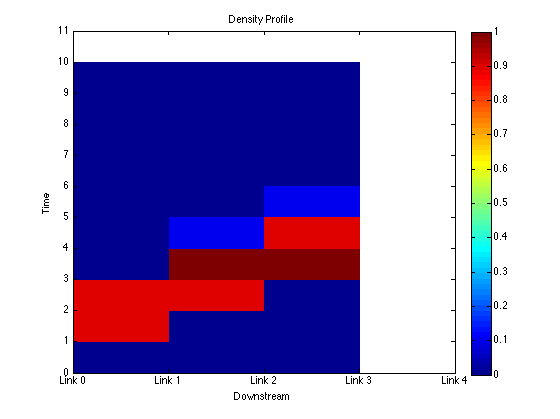
\includegraphics[width=60mm]{before.png}
\caption{No ramp metering}
\end{figure}
\end{minipage}\hfill
\begin{minipage}[t]{0.48\linewidth}
\begin{figure}[h]
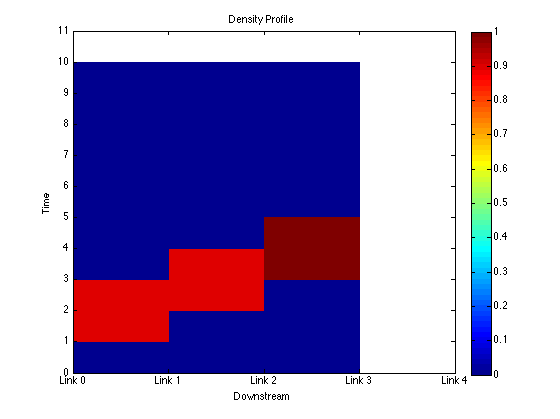
\includegraphics[width=60mm]{after.png}
\caption{Optimal ramp metering}
\end{figure}
\end{minipage}

\end{frame}

%-----------------------------------------------------------------------------------------------------------------------------------------------------------------
\begin{frame}{Numerical Results}

\begin{minipage}[t]{0.48\linewidth}
\begin{figure}[h]
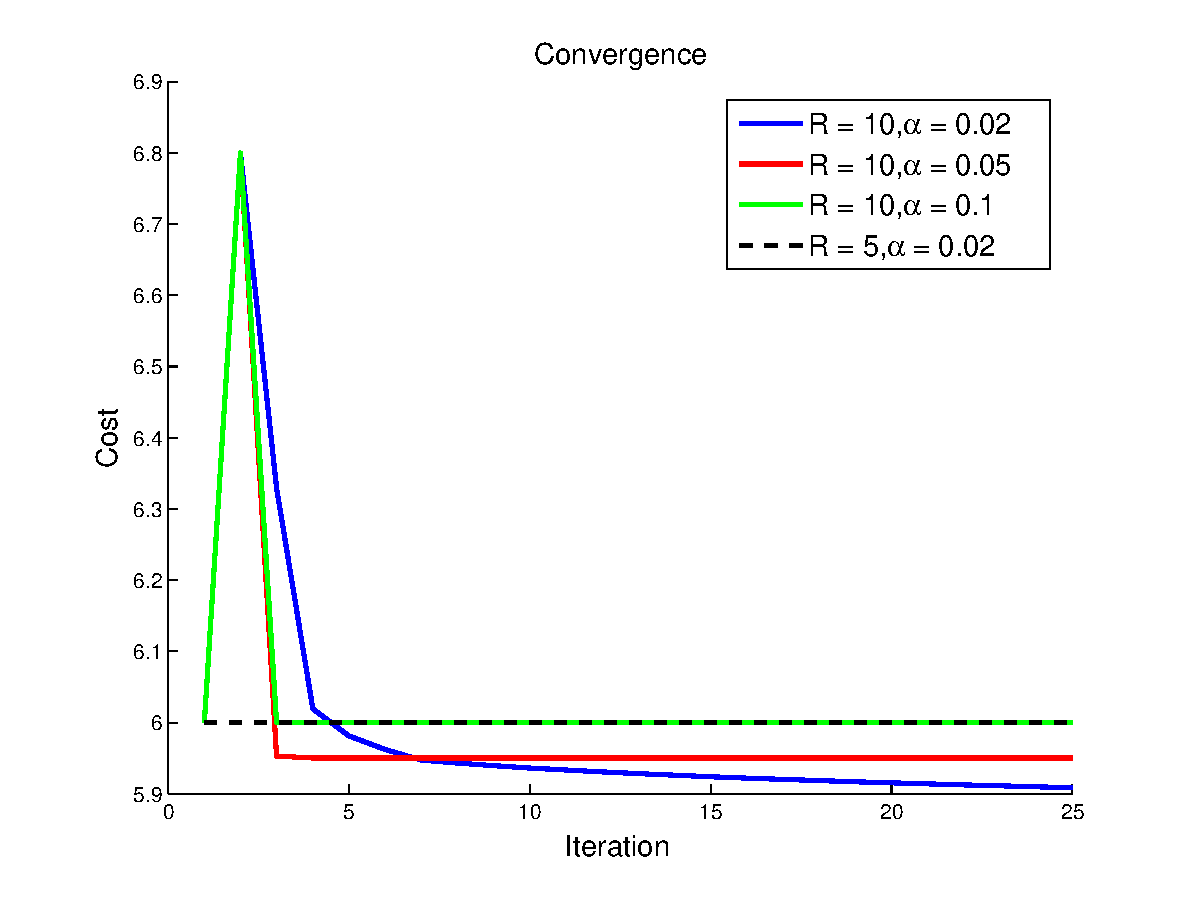
\includegraphics[width=60mm]{convergence.eps}
\end{figure}
\end{minipage}\hfill
\begin{minipage}[t]{0.48\linewidth}
\begin{figure}[h]
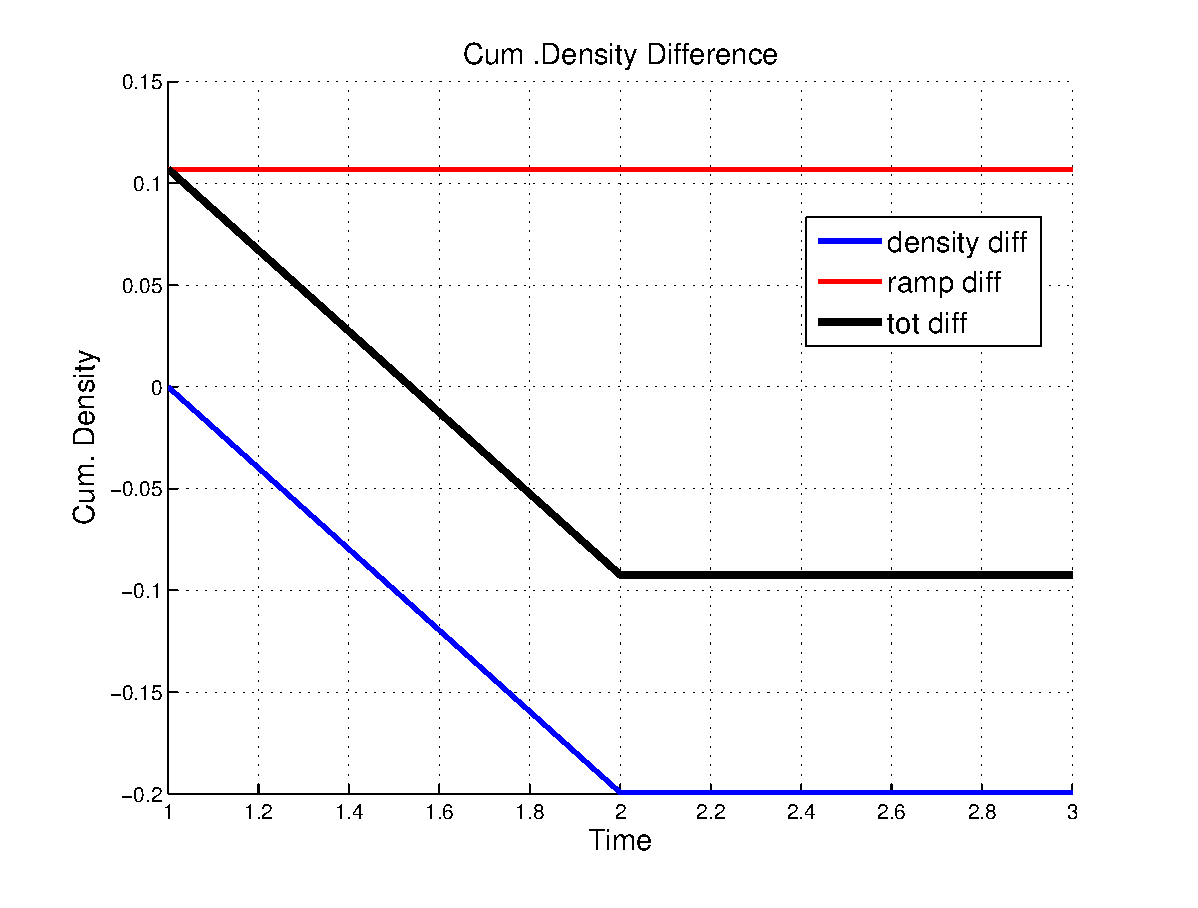
\includegraphics[width=60mm]{cumDiff}
\end{figure}
\end{minipage}

\end{frame}

%-----------------------------------------------------------------------------------------------------------------------------------------------------------------
\begin{frame}
\large
\begin{center}
Thank you.
\end{center}
\end{frame}

\end{document}
